\documentclass[cjk,slidestop,compress,mathserif,blue]{beamer}
%dvipdfm选项是关键,否则编译统统通不过
%beamer的颜色选项定义的是导航条和标题的颜色(即关键词structure的颜色)

%%%%%%%%%%%%%%%%仅限于XeTeX可使用的宏包%%%%%%%%%%%%%%%%%%%%%%%%%%%%
\usepackage{fontspec,xunicode,xltxtra,beamerthemesplit}
%\usepackage{beamerthemesplit}
\usepackage{xeCJK}
\setCJKmainfont[BoldFont=黑体, ItalicFont=楷体, BoldItalicFont=仿宋]{黑体}
%\setsansfont[Mapping=tex-text]{Adobe 黑体 Std}
%如果装了Adobe Acrobat,可在font.conf中配置Adobe字体的路径以使用其中文字体
%也可直接使用系统中的中文字体如SimSun,SimHei,微软雅黑 等
%原来beamer用的字体是sans family;注意Mapping的大小写,不能写错

%%%%%%%%   确定标题和导航条结构的框架     %%%%%%%%%%%%
\usepackage{beamerthemeshadow}                       %
%\usepackage{beamerthemeclassic}%导航条色与背景色一致%
%%%%%%%%%%%%%%%%%%%%%%%%%%%%%%%%%%%%%%%%%%%%%%%%%%%%%%
\setbeamerfont{roman title}{size={}}
%\usepackage{CJK} % CJK 中文支持                                  %
\usepackage{amsmath,amsthm,amsfonts,amssymb,bm}
\usepackage{mathrsfs}
\usepackage{xcolor}                                        %使用默认允许使用颜色
\usepackage{hyperref} 
\usepackage{graphicx}
\usepackage{subfigure}           %图片跨页

%\usepackage[numbers,sort&compress]{natbib} %紧密排列             %
\usepackage[sectionbib]{chapterbib}        %每章节单独参考文献   %
\usepackage{hypernat}                                                                         %
%\usepackage[dvipdfm,bookmarksopen=true,pdfstartview=FitH,CJKbookmarks]{hyperref}		%
\hypersetup{bookmarksnumbered,colorlinks,linkcolor=brown,citecolor=blue,urlcolor=red}         %
%参考文献含有超链接引用时需要下列宏包,注意与natbib有冲突        %
%\usepackage[dvipdfm]{hyperref}                                  %
%\usepackage{hypernat}                                           %
\newcommand{\upcite}[1]{\hspace{0ex}\textsuperscript{\cite{#1}}} %

%\useoutertheme{smoothbars}
\useinnertheme[shadow=true]{rounded}
\usetheme{Berkeley}                                          %主题式样
%\usetheme{Luebeck}

\usecolortheme{lily}                                        %颜色主题式样

\usefonttheme{professionalfonts}                           %字体主题样式宏包

%\beamertemplatetransparentcoveredhigh                      %使所有被隐藏的文本高度透明
\beamertemplatetransparentcovereddynamicmedium             %使所有被隐藏的文本完全透明,动态,动态的范围很小
\mode<presentation>
%\beamersetaveragebackground{gray}                          %设置背景颜色(单一色) 
\beamertemplateshadingbackground{green!10}{red!5}         %设置背景颜色(渐变色)

%在指定位置精确放置logo
\usepackage{tikz}
\usepackage{beamerfoils}
\usepackage{pgf}
\logo{\pgfputat{\pgfxy(11.68,0.15)}{
\includegraphics[height=1.01cm,viewport=0 0 140 120,clip]{Figures/BCC_logo-1.png}}\pgfputat{\pgfxy(10.502,-0.218)}{
\includegraphics[height=0.369cm,viewport=140 0 540 120,clip]{Figures/BCC_logo-1.png}}}
%\logo{\pgfputat{\pgfxy(11.68,0.15)}{
\includegraphics[height=0.95cm,viewport=0 0 510 360,clip]{Figures/Logo_Gainstrong.png}}\pgfputat{\pgfxy(10.333,-0.195)}{
\includegraphics[height=0.35cm,viewport=530 70 1100 218,clip]{Figures/Logo_Gainstrong.png}}}
%\MyLogo{
%	\pgfputat{\pgfxy(-50,-50)}{\pgfbox[right,base]{
\includegraphics[height=1cm]{Figures/BCC_logo-1.png}}}

%logo作为背景放置
%\setbeamertemplate{background}{
%	\pgfputat{\pgfxy(6.5,-0.5)}{\pgfbox[left,top]{\pgfimage[height=1.1cm]{Figures/BCC_logo-1.png}}}}

%\logo{}									%不显示logo

\begin{document}
%\begin{CJK*}{GBK}{song}
%\begin{CJK*}{GBK}{kai}
%beamer下不能用\songyi、\zihao等命令!
%\graphicspath{Figures/}

%-------------------------------PPT Title-------------------------------------
\title{原子尺度的材料模拟软件--ABINIT}
%-----------------------------------------------------------------------------

%----------------------------Author & Date------------------------------------
\author{北京市计算中心\;云平台\:姜骏}
\date{\textrm{2016.08.08-12}}
%\date{2013.09.10}
\frame{\titlepage}
%-----------------------------------------------------------------------------

%------------------------------------------------------------------------------列出全文 outline ---------------------------------------------------------------------------------
\section*{}
\frame[allowframebreaks]
{
  \frametitle{Outline}
%  \frametitle{\textcolor{mycolor}{\secname}}
  \tableofcontents%[current,currentsection,currentsubsection]
}
%在每个section之前列出全部Outline
%类似的在每个subsection之前列出全部Outline是\AtBeginSubsection[]
\AtBeginSection[]
{
  \frame<handout:0>
  {
    \frametitle{Outline}
%全部Outline中,本部分加亮
    \tableofcontents[current,currentsection]
  }
}

%------------------------------------------------------------------------------PPT main Body------------------------------------------------------------------------------------
\small
\section{ABINIT简介}
\frame
{
\frametitle{ABINIT概况}
\textrm{ABINIT}: 采用第一原理和分子动力学模拟材料性质的科学计算软件包
\begin{itemize}
	\item \textrm{ABINIT}使用赝势\textrm{(Pseudo Potential, PP)}和平面波\textrm{(Plane wave, PW)}或小波\textrm{(wavelet)}基组
	\item \textrm{ABINIT}采用密度泛函方法\textrm{(DFT)},可计算分子或周期体系的总能量、电荷密度和电子能带结构等信息
	\item \textrm{ABINIT}还可以按\textrm{H-F}力和应力来优化体系的几何结构,或根据原子受力进行分子动力学模拟,计算动力学矩阵、\textrm{Born}有效电荷及介电张量
	\item 在含时密度泛含理论的框架下可以计算分子体系的激发态,也可以基于多体微扰论(\textrm{GW}近似)来处理激发态
\end{itemize}
除主要计算模块,\textrm{ABINIT}还提供一些工具模块用来处理结果和数据
}

\section{ABINIT的使用}
\frame
{
	\frametitle{ABINIT的运行}
	完成\textrm{ABINIT}计算,需要准备三个文件
\begin{itemize}
        \setlength{\itemsep}{15pt} %调整10mm 
		\item \textcolor{red}{x.in}\hspace{3pt}(存放计算所需要的计算参数)\\
			注意:\begin{itemize}
				\item 负值的数值与符号间不能有空格
				\item 不允许使用Tab键作分隔符
				\item 每一行的字符数不超过132个
			\end{itemize}
		\item \textcolor{red}{赝势文件}\hspace{3pt}(\textrm{ABINTI}官网可下载,也可通过\textrm{AtomPAW}生成)
		\item \textcolor{red}{x.files}\hspace{3pt}(指定计算中输入、输出文件和赝势文件的位置)
\end{itemize}
	\vspace{15pt}
	运行\textrm{ABINIT}计算命令:\hspace{10pt}
	\textcolor{red}{abinit} < x.files >\& log 
}

\frame
{
	\frametitle{ABINIT的输入文件-1}
	\textrm{x.in}控制着整个计算的过程和精度,相当于\textrm{VASP}软件的\textrm{INCAR}、\textrm{POSCAR}和\textrm{KPOINTS}的“综合体”\\
	Si(Diamond Structure)计算的输入文件\textcolor{red}{Si.in}:
\begin{figure}[h!]
\centering
\vspace{-4.5pt}
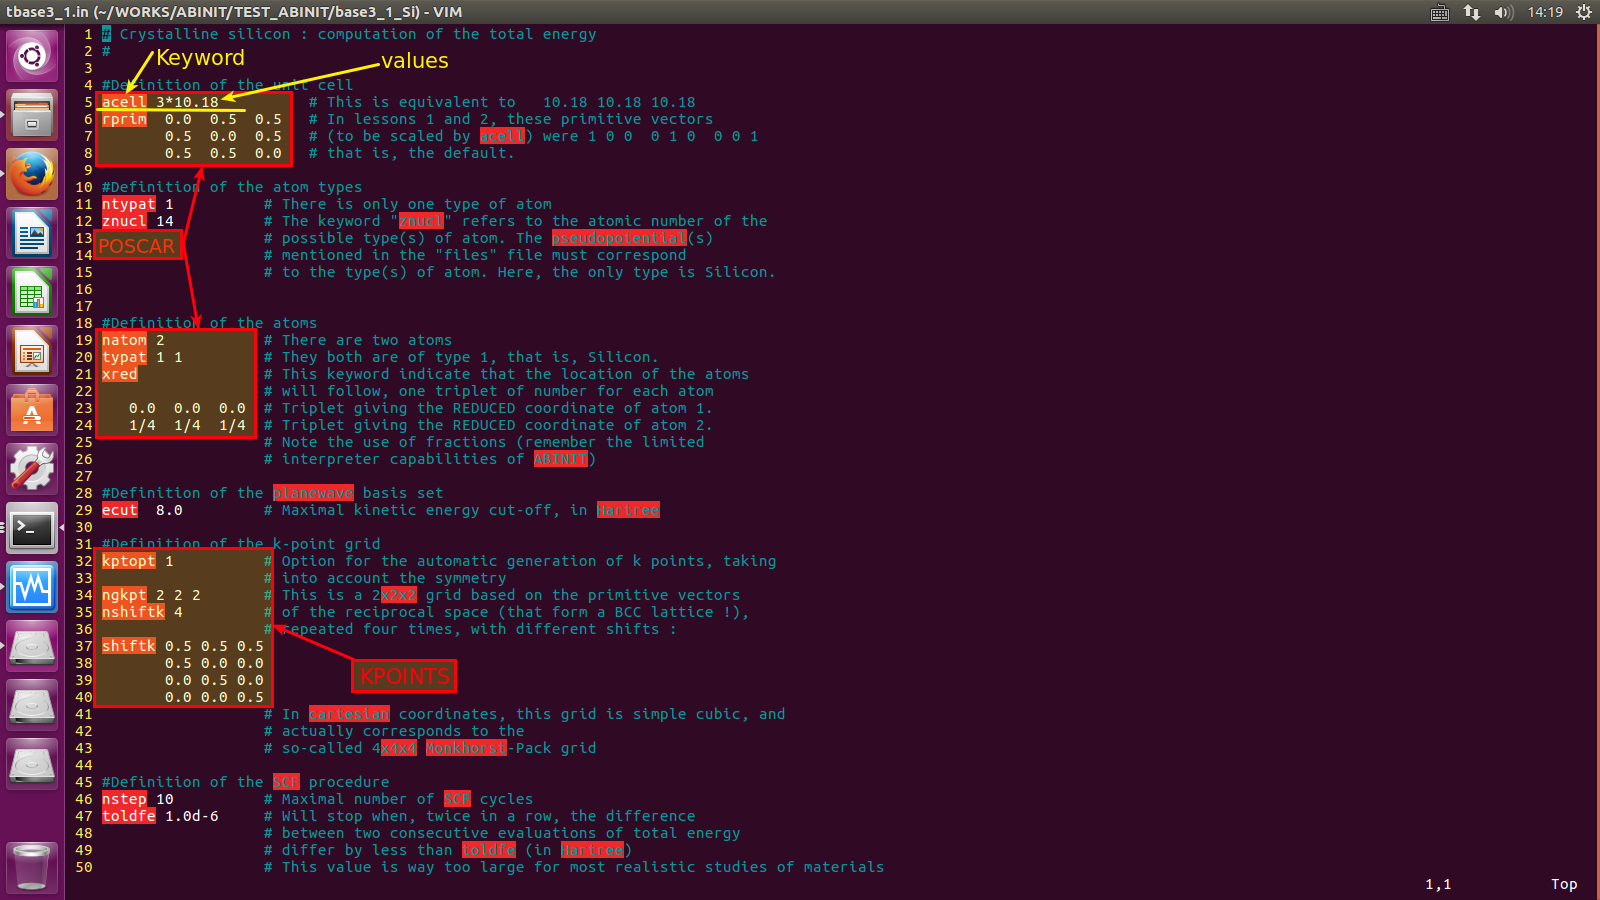
\includegraphics[height=0.6524\textwidth,width=0.85\textwidth,viewport=70 360 775 875,clip]{Figures/2016-06-28_Si-1.png}
\caption{\textrm{ABINIT}的Si.in}
\label{X.in-1}
\end{figure}
}

\frame
{
	\frametitle{ABINIT的输入文件-1}
\begin{figure}[h!]
\centering
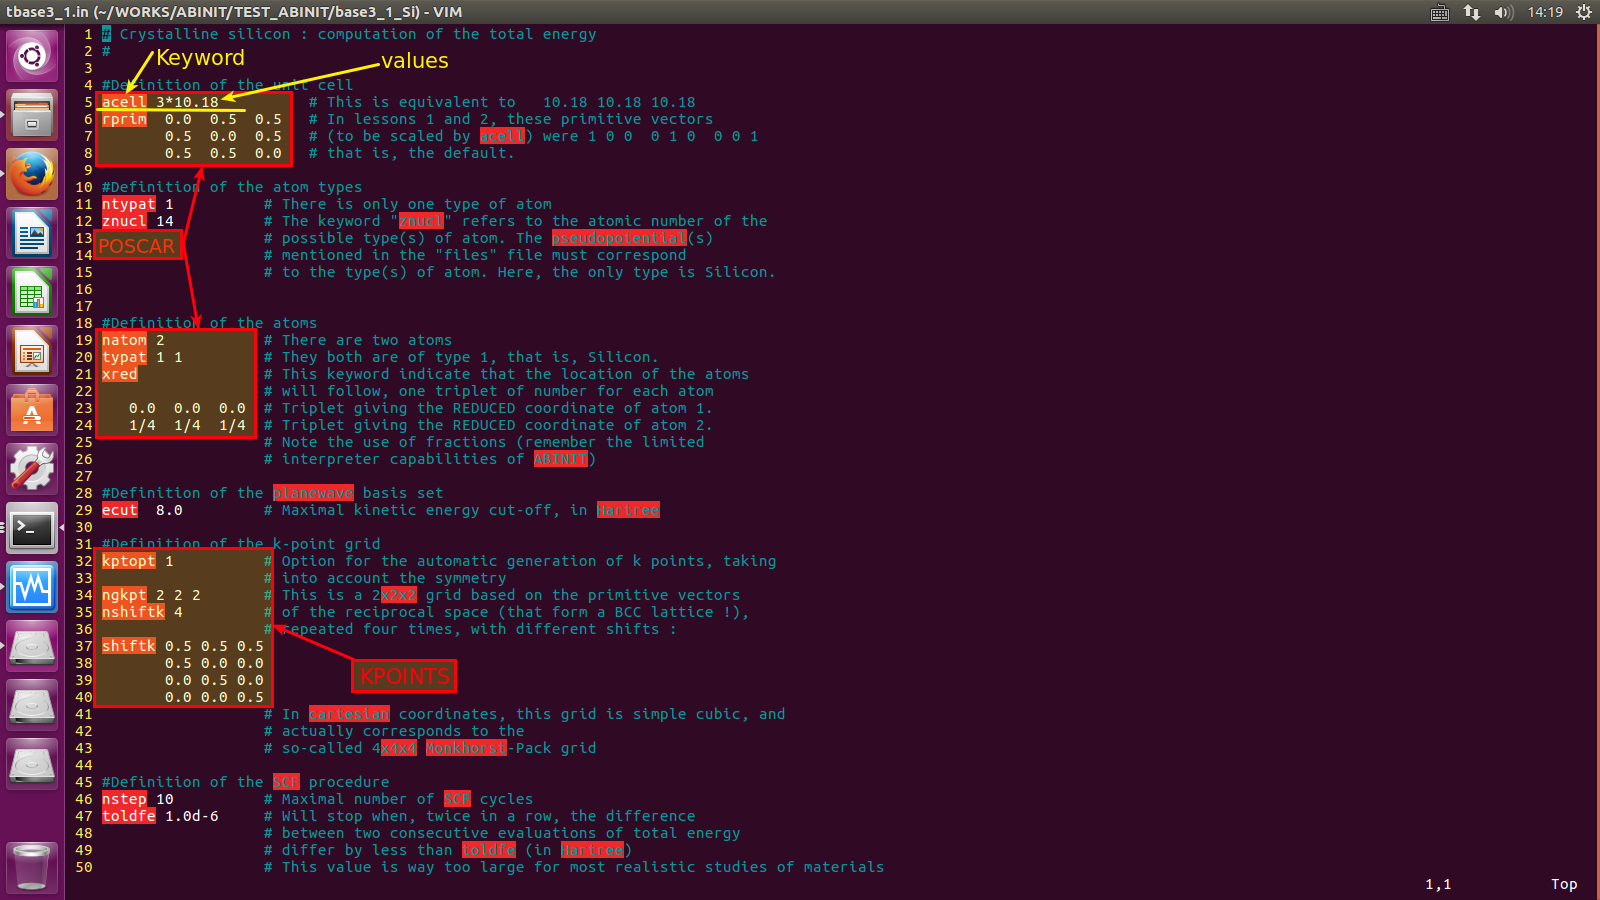
\includegraphics[height=0.5487\textwidth,width=1.04\textwidth,viewport=70 20 900 432,clip]{Figures/2016-06-28_Si-1.png}
\caption{\textrm{ABINIT}的Si.in}
\label{X.in-2}
\end{figure}
}

\frame
{
	\frametitle{ABINIT的输入文件-1}
\begin{figure}[h!]
\centering
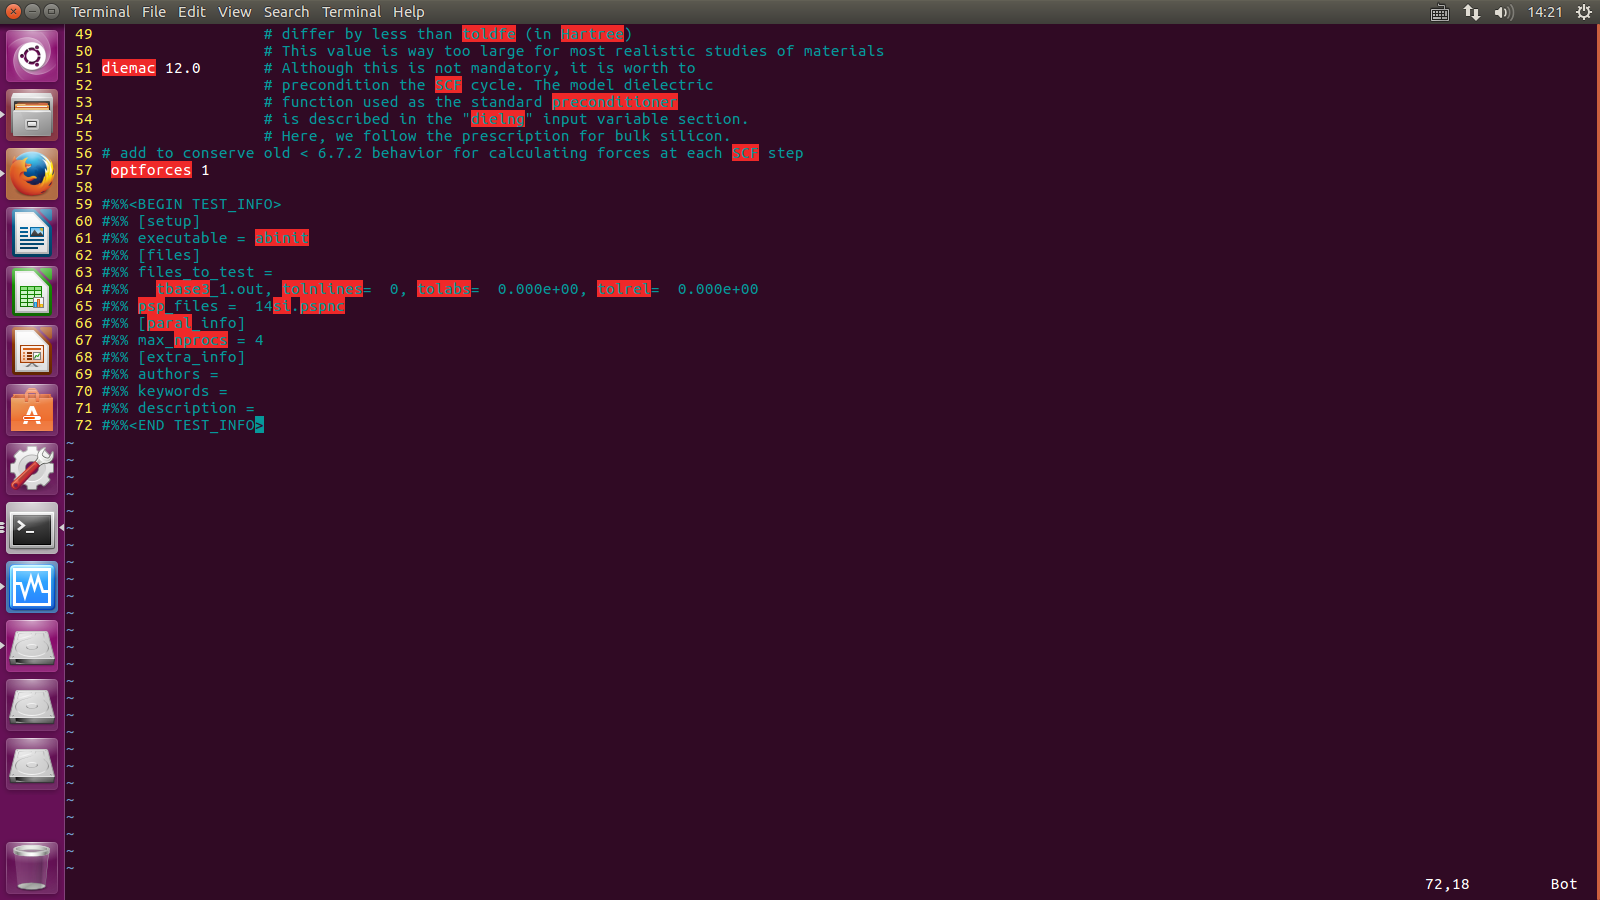
\includegraphics[height=0.5487\textwidth,width=0.90\textwidth,viewport=70 400 825 875,clip]{Figures/2016-06-28_Si-2.png}
\caption{\textrm{ABINIT}的Si.in}
\label{X.in-3}
\end{figure}
}

\frame
{
	\frametitle{ABINIT的输入文件-2}
\begin{figure}[h!]
\centering
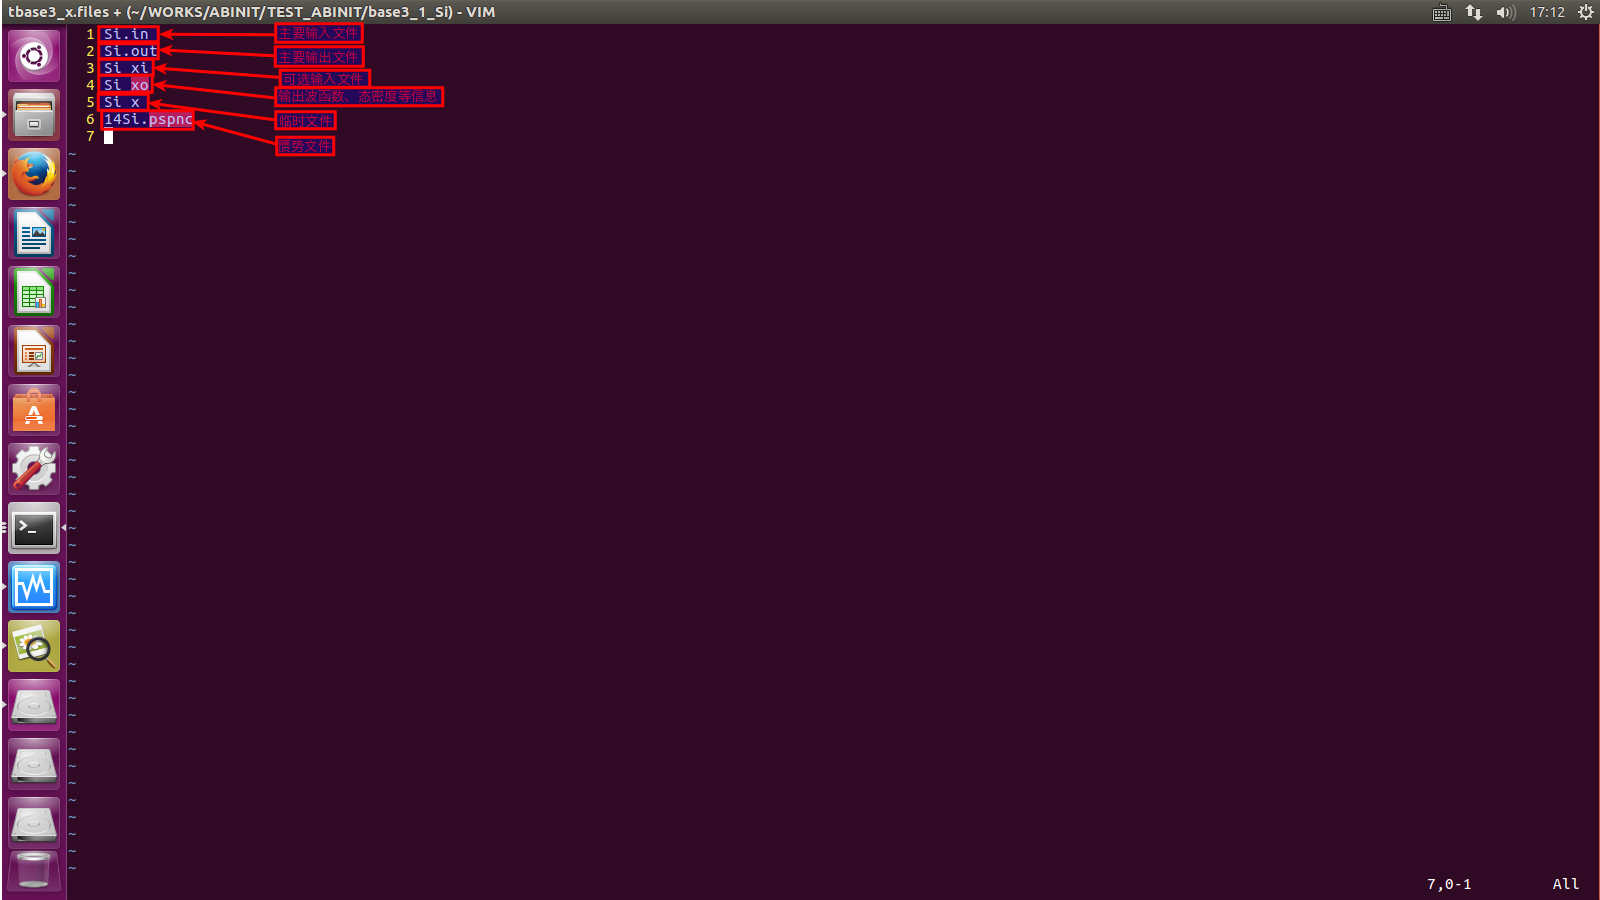
\includegraphics[height=0.5524\textwidth,width=0.85\textwidth,viewport=70 600 475 875,clip]{Figures/2016-06-28_Si-3.png}
\caption{\textrm{ABINIT}的Si.files}
\label{X.files}
\end{figure}
}

\frame
{
	\frametitle{ABINIT的输入文件-3}
\begin{figure}[h!]
\centering
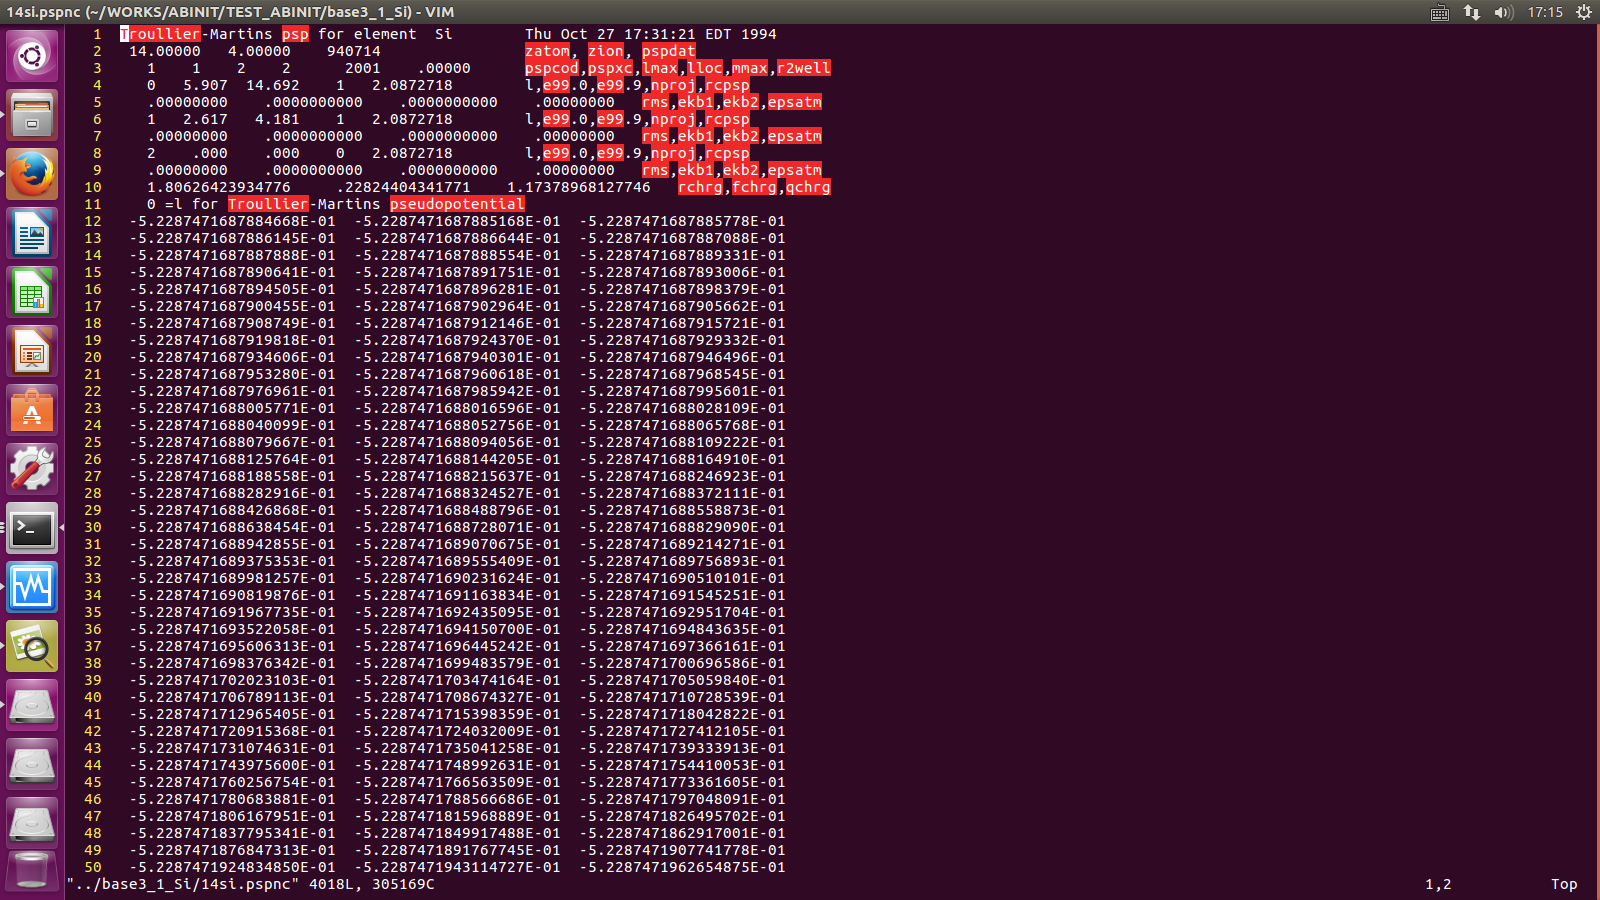
\includegraphics[height=0.6087\textwidth,width=0.95\textwidth,viewport=70 400 875 875,clip]{Figures/2016-06-28_Si-4.png}
\caption{\textrm{ABINIT}的Si.in}
\label{X.potential}
\end{figure}
}

\section{密度泛函理论}       %Bookmark
\frame
{
	\frametitle{\textrm{Thomas-Fermi}模型} 
	1927年,\textrm{Thomas}和\textrm{Fermi}基于均匀电子气模型上建立\textrm{Thomas-Fermi}模型,\textcolor{blue}{体系能量可用}\textcolor{red}{电子密度}\textcolor{blue}{表示}:
	\begin{itemize}
		\item 动能表达式
			$$T_{\mathrm{TF}}[\rho(\vec r)]=\dfrac3{10}(3\pi^2)^{\frac23}\int\rho^{\frac53}(\vec r)\mathrm{d}\vec r$$
		\item 外势$V_{ext}(\vec r)$下电子体系的能量泛函表达式为
			\begin{displaymath}
				\begin{aligned}
					E_{\mathrm{TF}}[\rho(\vec r)]=&\dfrac3{10}(3\pi^2)^{\frac23}\int\rho^{\frac53}(\vec r)\mathrm{d}\vec r\\
					&-Z\int\dfrac{\rho(\vec r)}{r}\mathrm{d}\vec r+\dfrac12\int\int\dfrac{\rho(\vec r_1)\rho(\vec r_2)}{|\vec r_2-\vec r_1|}\mathrm{d}\vec r_1\mathrm{d}\vec r_2
				\end{aligned}
			\end{displaymath}
		\item \textrm{Thomas-Fermi}模型完全没有考虑电子的交换-相关作用
	\end{itemize}
}

\frame
{
	\frametitle{\textrm{Thomas-Fermi-Dirac}模型} 
	1930年,\textrm{Dirac}将\textrm{Thomas-Fermi}模型修正,用局域密度近似考虑电子交换作用
			\begin{displaymath}
				\begin{aligned}
					E_{\mathrm{TFD}}[\rho(\vec r)]=&\dfrac3{10}(3\pi^2)^{\frac23}\int\rho^{\frac53}(\vec r)\mathrm{d}\vec r-Z\int\dfrac{\rho(\vec r)}{r}\mathrm{d}\vec r\\
					&+\dfrac12\int\int\dfrac{\rho(\vec r_1)\rho(\vec r_2)}{|\vec r_2-\vec r_1|}\mathrm{d}\vec r_1\mathrm{d}\vec r_2-\dfrac34\bigg(\dfrac3{\pi}\bigg)^{\frac13}\int\rho^{\frac43}(\vec r)\mathrm{d}\vec r
				\end{aligned}
			\end{displaymath}
			\begin{itemize}
				\item 在总电子数守恒约束条件
					$$\int\rho(\vec r)\mathrm{d}\vec r=N$$
					下,能量泛函$E_{\mathrm{TFD}[\rho(\vec r)]}$对密度$\rho(\vec r)$的变分极小获得体系的基态密度和基态能量
			\end{itemize}
}

\frame
{
	\frametitle{\textrm{Thomas-Fermi}模型}
	\begin{itemize}
		\item \textrm{Thomas-Fermi}模型用电子密度代替波函数描述问题是极大的简化,但模型过于粗糙:\\
%			\begin{enumerate}
%				\item 以均匀电子气的密度得到动能的表达式
%				\item 完全忽略电子间的交换-相关作用
%			\end{enumerate}
			不能正确描述相互作用电子体系的基本特征,如原子的壳层结构
		\item \textrm{Thomas-Fermi}模型虽不够精确,但可以通过引入修正项校正:
			\textrm{Dirac}交换泛函 $$E_X[\rho(\vec r)]=-\dfrac34\bigg(\dfrac3{\pi}\bigg)^{\frac13}\int\rho^{\frac43}(\vec r)\mathrm{d}\vec r$$
			\textrm{Wigner}相关泛函 $$E_C[\rho(\vec r)]=-0.056\int\dfrac{\rho^{\frac43}(\vec r)}{0.079+\rho^{\frac13}(\vec r)}\mathrm{d}\vec r$$
	\end{itemize}
	\textrm{Thomas-Fermi}模型为密度泛函理论\textrm{(DFT)}提供了重要的启示
}

\frame                               %
{
\frametitle{密度泛函理论(\textrm{DFT})} %Slide Page Title
%   \secname
与传统的量子力学方法不同,密度泛函理论的基本变量是体系的基态电子密度。%通过体系的电子密度而非波函数确定体系的基态能量。
\begin{itemize}%[+-| alert@+>]
	\item 密度泛函理论的基石:\textrm{Hohenberg-Kohn}定理\upcite{PR136-B864_1964}
\vskip 5pt
\begin{itemize}%[+-| alert@+>]
   \setlength{\itemsep}{8pt}
 \item $E[\rho]=F_{\mathrm{HK}}[\rho]+\displaystyle\int\rho(\vec{r})v(\vec{r})\textrm{d}^{3}\vec{r}$ \\
\vskip 5pt 其中$F_{\mathrm{HK}}[\rho]=\underset{\Psi\to\rho}{\mathrm{Min}}\langle\Psi[\rho]|\hat{T}+\hat{W}|\Psi[\rho]\rangle$
是普适的泛函表达式。%,指明多电子体系的基态性质与基态密度间存在一一对应关系
     \textrm{\small{第一定理表明多电子体系的性质完全由体系的基态密度决定}}
   \item 如果$\tilde\Psi\neq\Psi$,
     $E[\tilde\rho]\geqslant E[\rho_0]$\\
     \textrm{\small{第二定理指出基态总能量泛函在体系基态电子密度处取极小值}}
   \end{itemize}
%\textrm{\small{第二定理指出基态总能量泛函在体系基态电子密度处取极小值}}
\vskip 8pt
 \item 密度泛函理论的优越性:用密度($\rho$)代替波函数($\Psi$)描述体系
\vskip 5pt
 \item 密度泛函理论的困难:能量密度泛函的精确形式未知
   \end{itemize}
}
\frame                               %
{
\frametitle{密度泛函理论(\textrm{DFT})}
\textrm{Kohn-Sham}方程\upcite{PR140-A1133_1965}:无相互作用体系+交换-相关能
$$(T_S+V_{e\!f\!f})|\varphi_i\rangle=\varepsilon_i|\varphi_i\rangle,\quad i=1,\cdots,N,\dots$$
其中$V_{e\!f\!f}(\vec r)=v(\vec r)+\displaystyle\int w(\vec r,\vec r\,')\rho(\vec r\,')d^3\vec r+\dfrac{\delta E_{XC}}{\delta\rho(\vec r)}$
\vskip 10pt
\textrm{Kohn-Sham}方程是形式上的单粒子方程
\vskip 20pt
\textrm{Kohn-Sham}方程的实质:\\将动能泛函的主要部分分离出来,剩余部分放在交换相关能中
}
%  \beamertemplateshadingbackground{blue!10}{yellow!10}
\frame                               %
{
\frametitle{交换-相关能密度泛函}
\begin{minipage}[b]{0.72\linewidth}
 \hspace*{-15pt}
 \begin{itemize}%[+-| alert@+>]
	 \setlength{\itemsep}{10pt}
 \item \textrm{LDA}:泛函只与密度分布的局域值有关
 \item \textrm{GGA}:泛函依赖:局域密度及其梯度
 \item $meta$-\textrm{GGA}:泛函依赖的变量还有动能密度
 \item 杂化(\textrm{hybrid})泛函:泛函与占据轨道有关
 \item 其他的交换-相关能泛函
 \item<1-> 完全非局域泛函:理想泛函,不现实
 \end{itemize}
\end{minipage}
\hfill
\begin{minipage}[b]{0.26\linewidth}
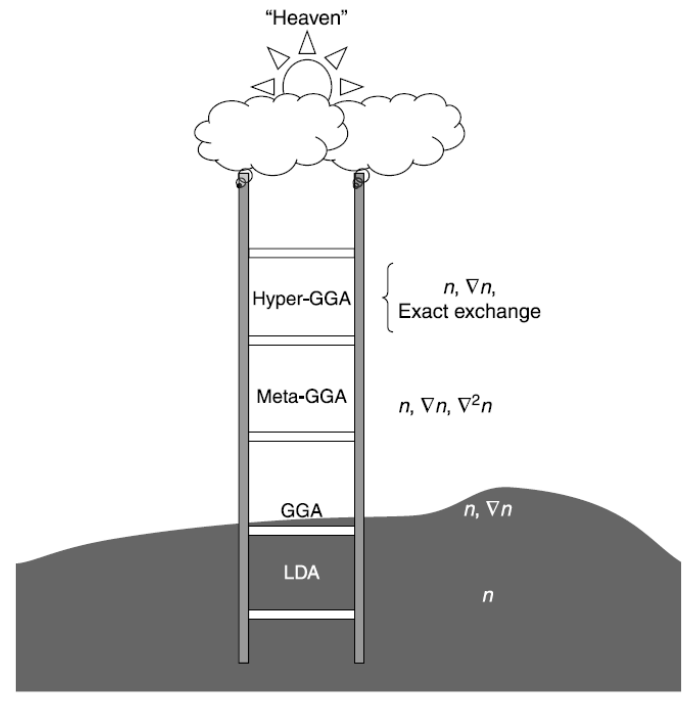
\includegraphics[height=1.7in,width=3.18in,viewport=10 5 1380 700,clip]{Figures/Jacobi-ladder.png}\\
{\small \textcolor{red}{\textrm{Jacob's ladder}}}
\end{minipage}
% \begin{itemize}%[+-| alert@+>]
%\item 交换-相关能密度泛函
}

\frame                               %
{
	\frametitle{近似能量泛函$E_{\mathrm{XC}}[\rho]$的主要问题}
\vskip 20pt
\begin{enumerate}%[+-| alert@+>]
   \setlength{\itemsep}{30pt}
 \item  密度是整体变量:电子自相互作用抵消不净%\quad\textrm{(LDA+U)}方法的校正%(\textrm{LDA+U})
 \item  电子相关:简并和近简并基态能量的表示不合理
 \item  渐近行为:处理弱相互作用体系的误差大
 \end{enumerate}
}

\frame                               %
{
	\frametitle{\textrm{Kohn-Sham}方程}
\begin{figure}[h!]
\centering
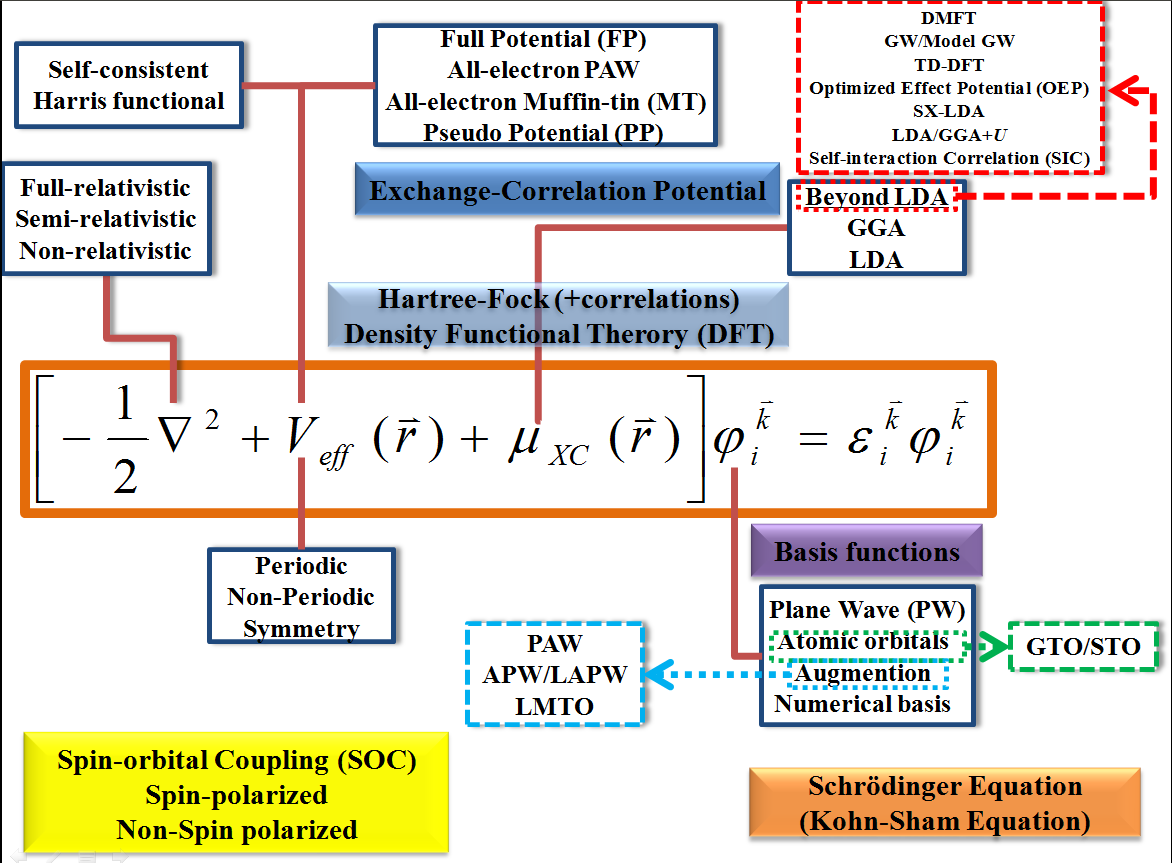
\includegraphics[height=2.3in,width=3.0in,viewport=1 5 780 580,clip]{Figures/DFT.png}
\caption{\small \textrm{The Analysis of Kohn-Sham equation.}}%(与文献\cite{EPJB33-47_2003}图1对比)
\label{DFT}
\end{figure}
}

%\section{Induction on DFT and solid-state physics}       %Bookmark
\section{固体能带与赝势}       %Bookmark
\frame
{
%\frametitle{The Bloch theorem}
\frametitle{固体能带理论}
\begin{itemize}%[+-| alert@+>]
   \setlength{\itemsep}{8pt}
   \item 固体能带理论\upcite{Huang_Han}是固体电子理论的基础,形式上是单电子理论:
    $$\hat H |\psi_i^{\vec k}(\vec r)\rangle=\bigg[-\dfrac{\hbar^2}{2m}\nabla^2+V(\vec r)\bigg]|\psi_i^{\vec k}(\vec r)\rangle=\epsilon_i(\vec k)|\psi_i^{\vec k}(\vec r)\rangle$$
  \item \textrm{Bloch}定理:
%   \item \textrm{periodic potential:} $$V(\vec r)=V(\vec r+\vec R_n)$$
%     \textrm{Here,} $\vec R_n=n\vec R$
%   \item \textrm{Bloch theorem:}$$\psi_{\vec k}(\vec r)=\textrm{e}^{\textrm i\vec k\cdot\vec r}u_{\vec k}(\vec r)$$
%     \textrm{Here, $u_{\vec k}(\vec r)$ is a periodic function with the same periodicity as $V(\vec r)$, i.e., $u_{\vec k}(\vec r)=u_{\vec k}(\vec r+\vec R_n)$, then Bloch theorem could reads as:}
%     $$\psi_{\vec k}(\vec r+\vec R_n)=\textrm{e}^{\textrm i\vec k\cdot\vec R_n}\psi_{\vec k}(\vec r)$$
具有平移周期性的理想晶体,势能$V(\vec r)$满足$$V(\vec r)=V(\vec r+\vec R_n)$$
体系的波函数满足\textrm{Bloch}波函数形式:$$\psi_{\vec k}(\vec r)=\textrm{e}^{i\vec k\cdot\vec r}u_{\vec k}(\vec r)$$
是平面波和周期函数的乘积。$u(\vec r)$与势能有相同的周期。即$$u_{\vec k}(\vec r)=u_{\vec k}(\vec r+\vec R_n)$$
  \item 能带理论相当于分子轨道理论
%   \setlength{\itemsep}{30pt}
\item \textrm{Bloch}函数反映了波函数在周期性势场下的变化规律。
\end{itemize}
}

\frame
{
\frametitle{固体能带理论}
简并态微扰理论引起的能带裂分
\begin{figure}[h!]
\centering
%\hspace*{-10pt}
%\vspace*{-1.1in}
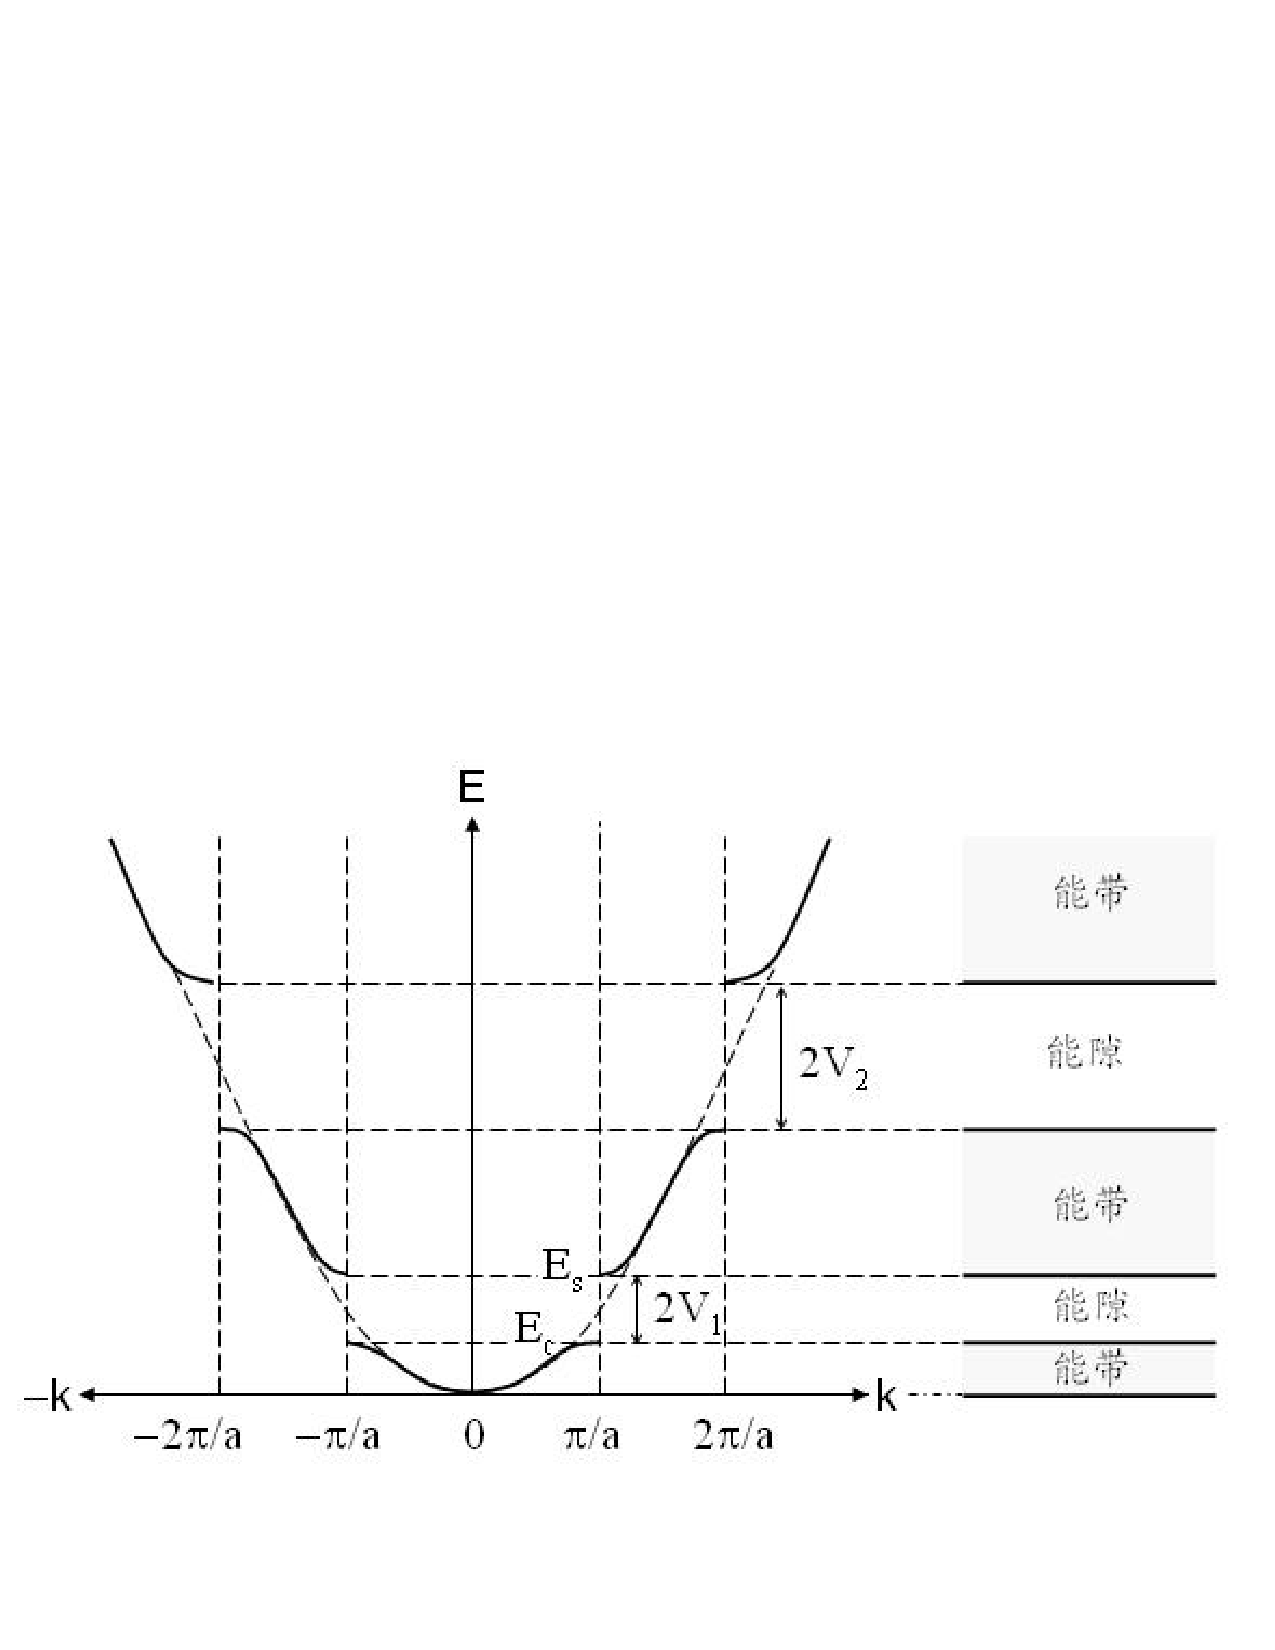
\includegraphics[height=2.1in,width=3.8in,viewport=10 90 570 380,clip]{Figures/Band_Gap.pdf}
\caption{\small \textrm{The Band-structure from free-electron gas.}}%
\label{Band-Structure-1}
\end{figure} 
}

\frame
{
\frametitle{固体能带理论}
从分子轨道到能带
\begin{figure}[h!]
\centering
\hspace*{-0.29in}
\vspace*{-0.1in}
\subfigure[一维$\mathrm{H}$原子链]{
\label{fig:Hydrogen-1D}
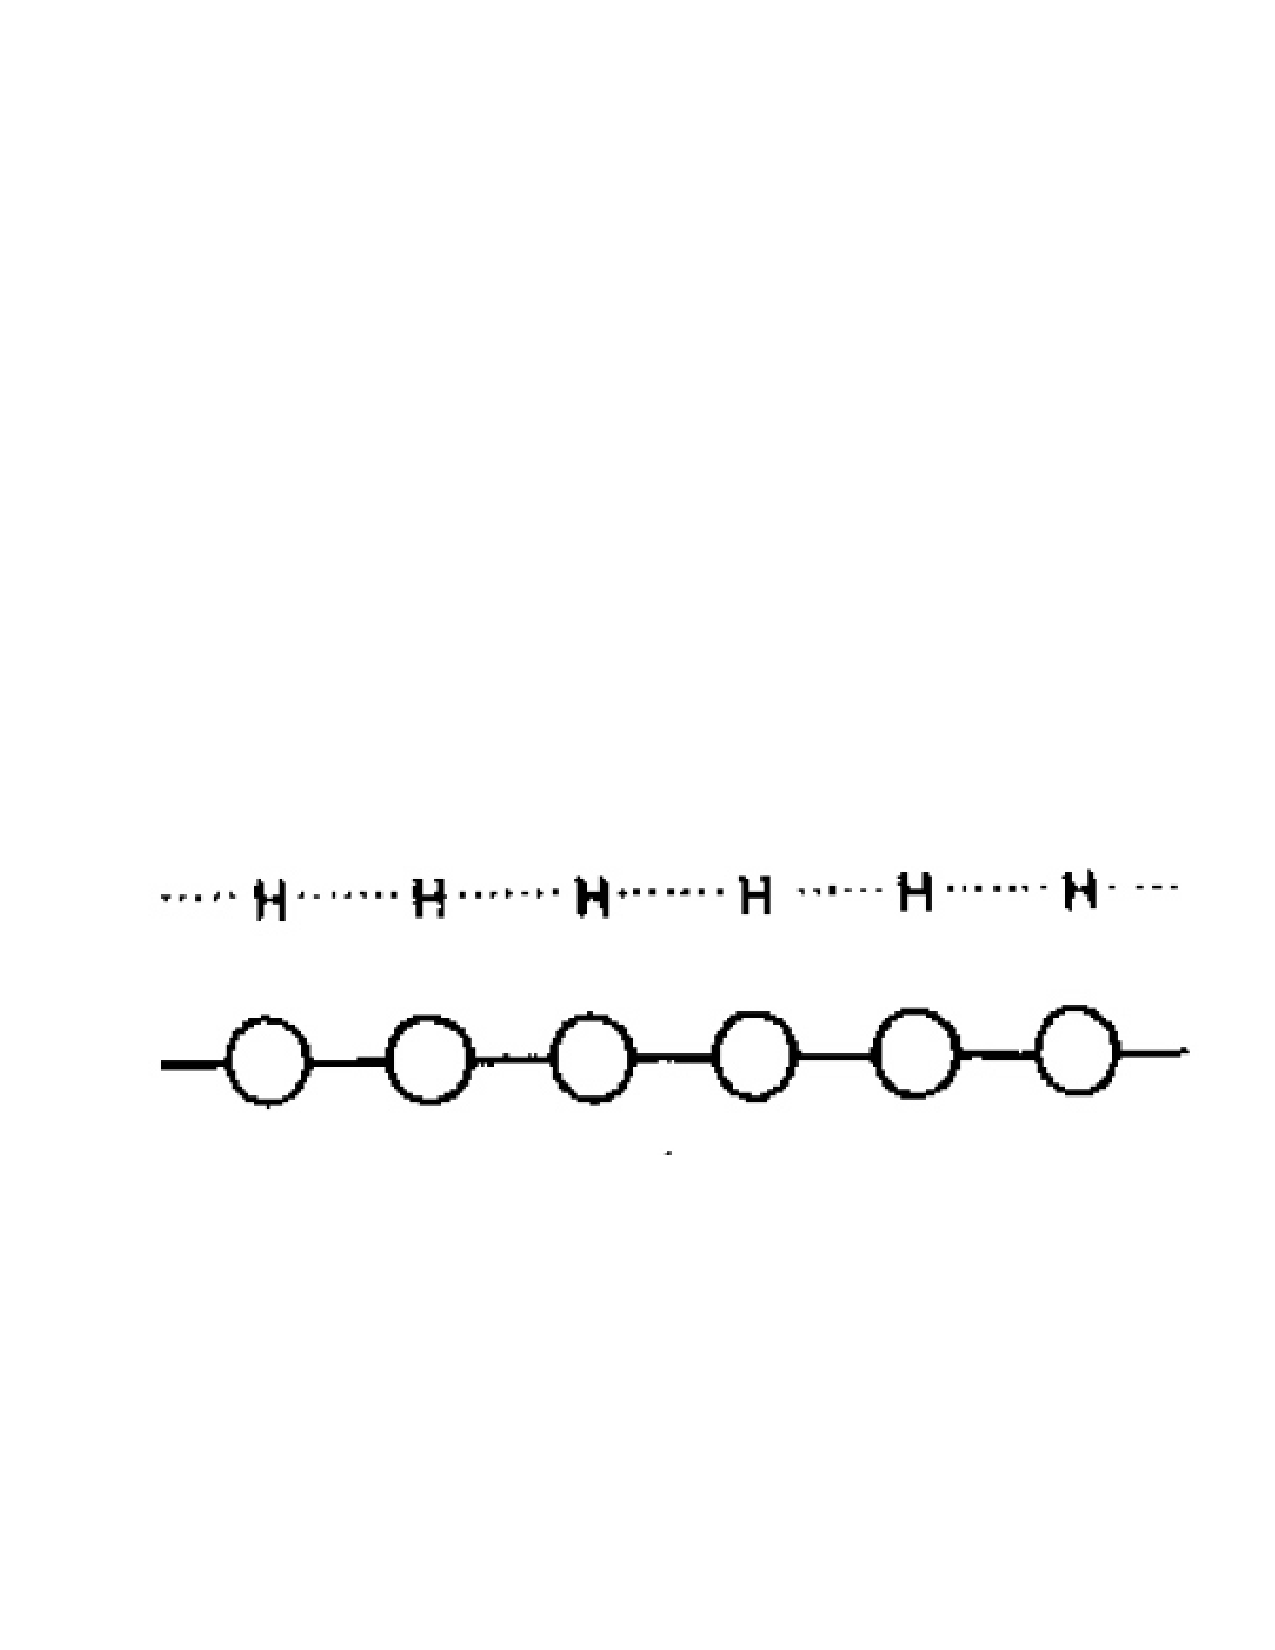
\includegraphics[height=0.25in,width=1.1in,viewport=70 255 570 375,clip]{Figures/Hydrogen-1D.pdf}}
\subfigure[$\mathrm{H}_n$分子轨道]{
\label{fig:Hydrogen-2-n}
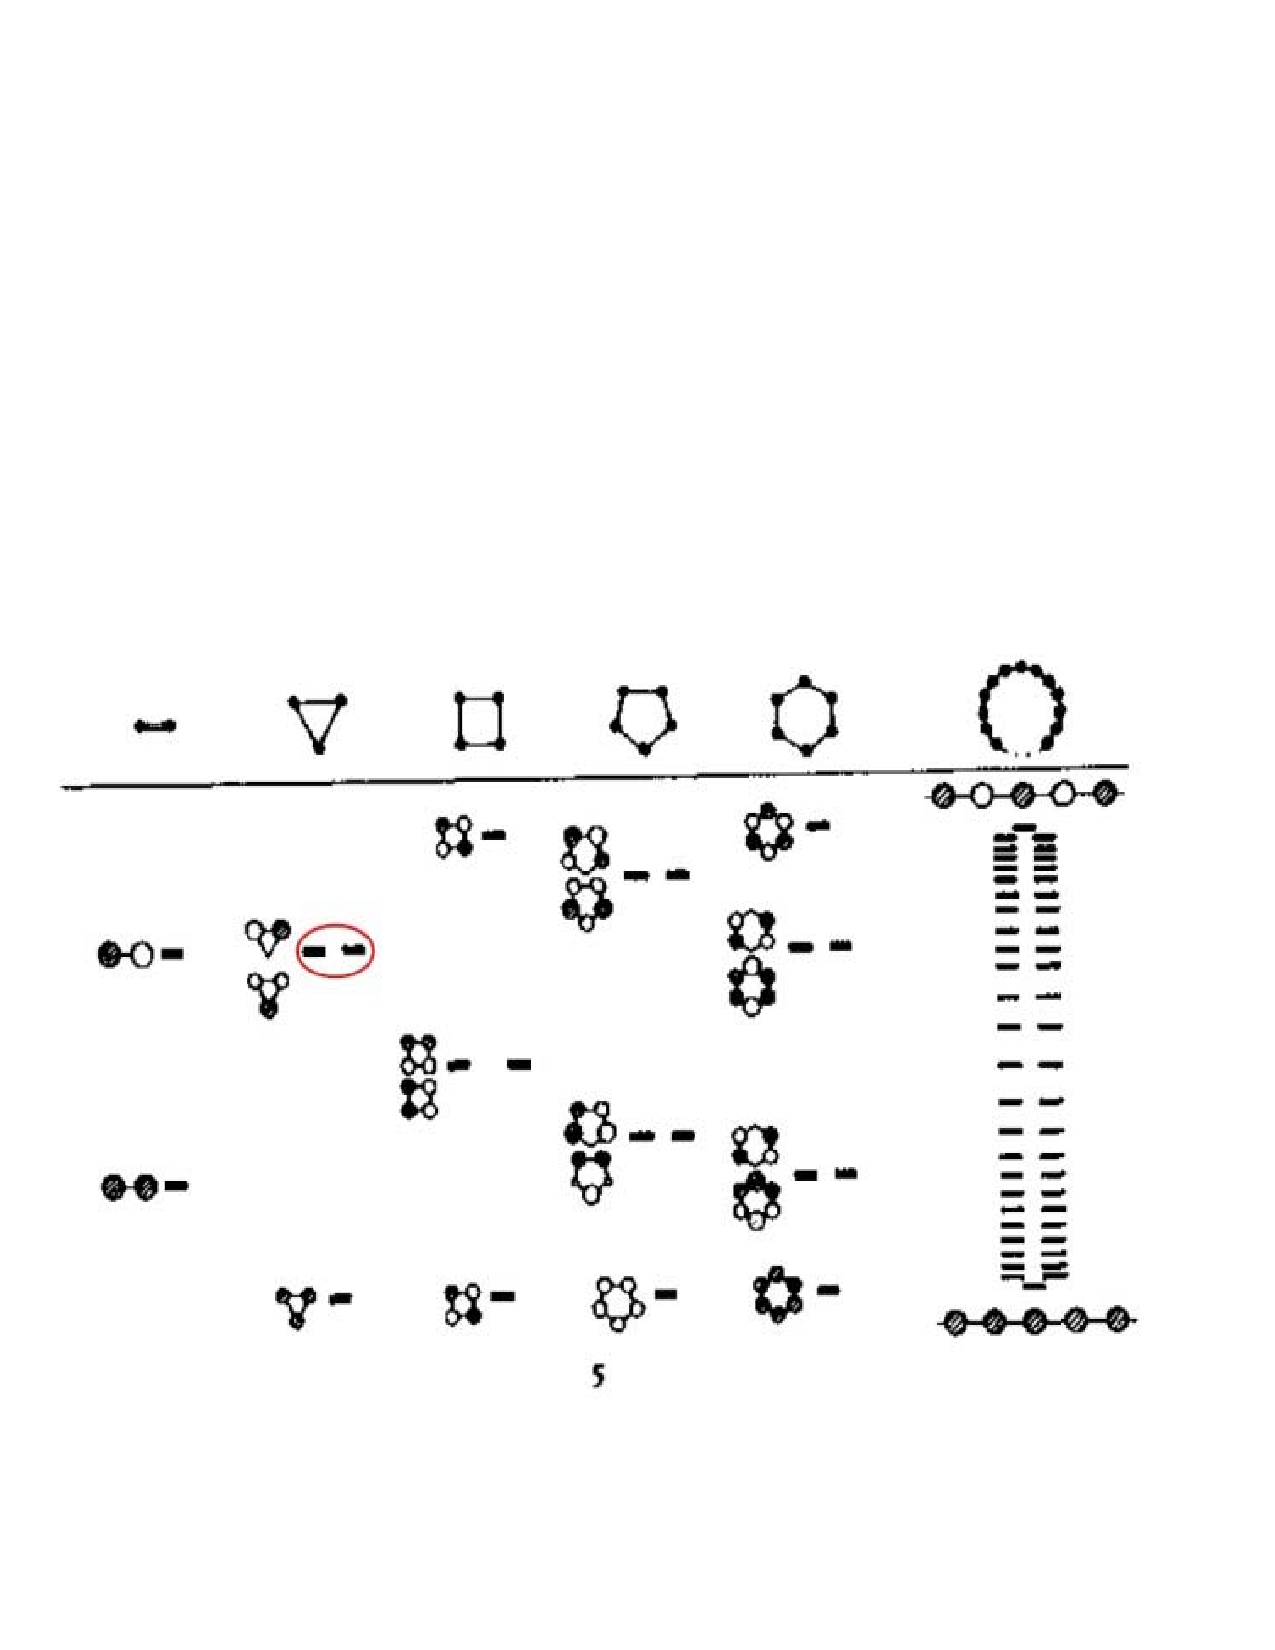
\includegraphics[height=0.8in,width=1.5in,viewport=30 140 545 480,clip]{Figures/Hydrogen-Mol-Orbital.pdf}}
\subfigure[分子波函数]{
\label{fig:Hydrogen-Psi}
\vspace*{-0.2in}
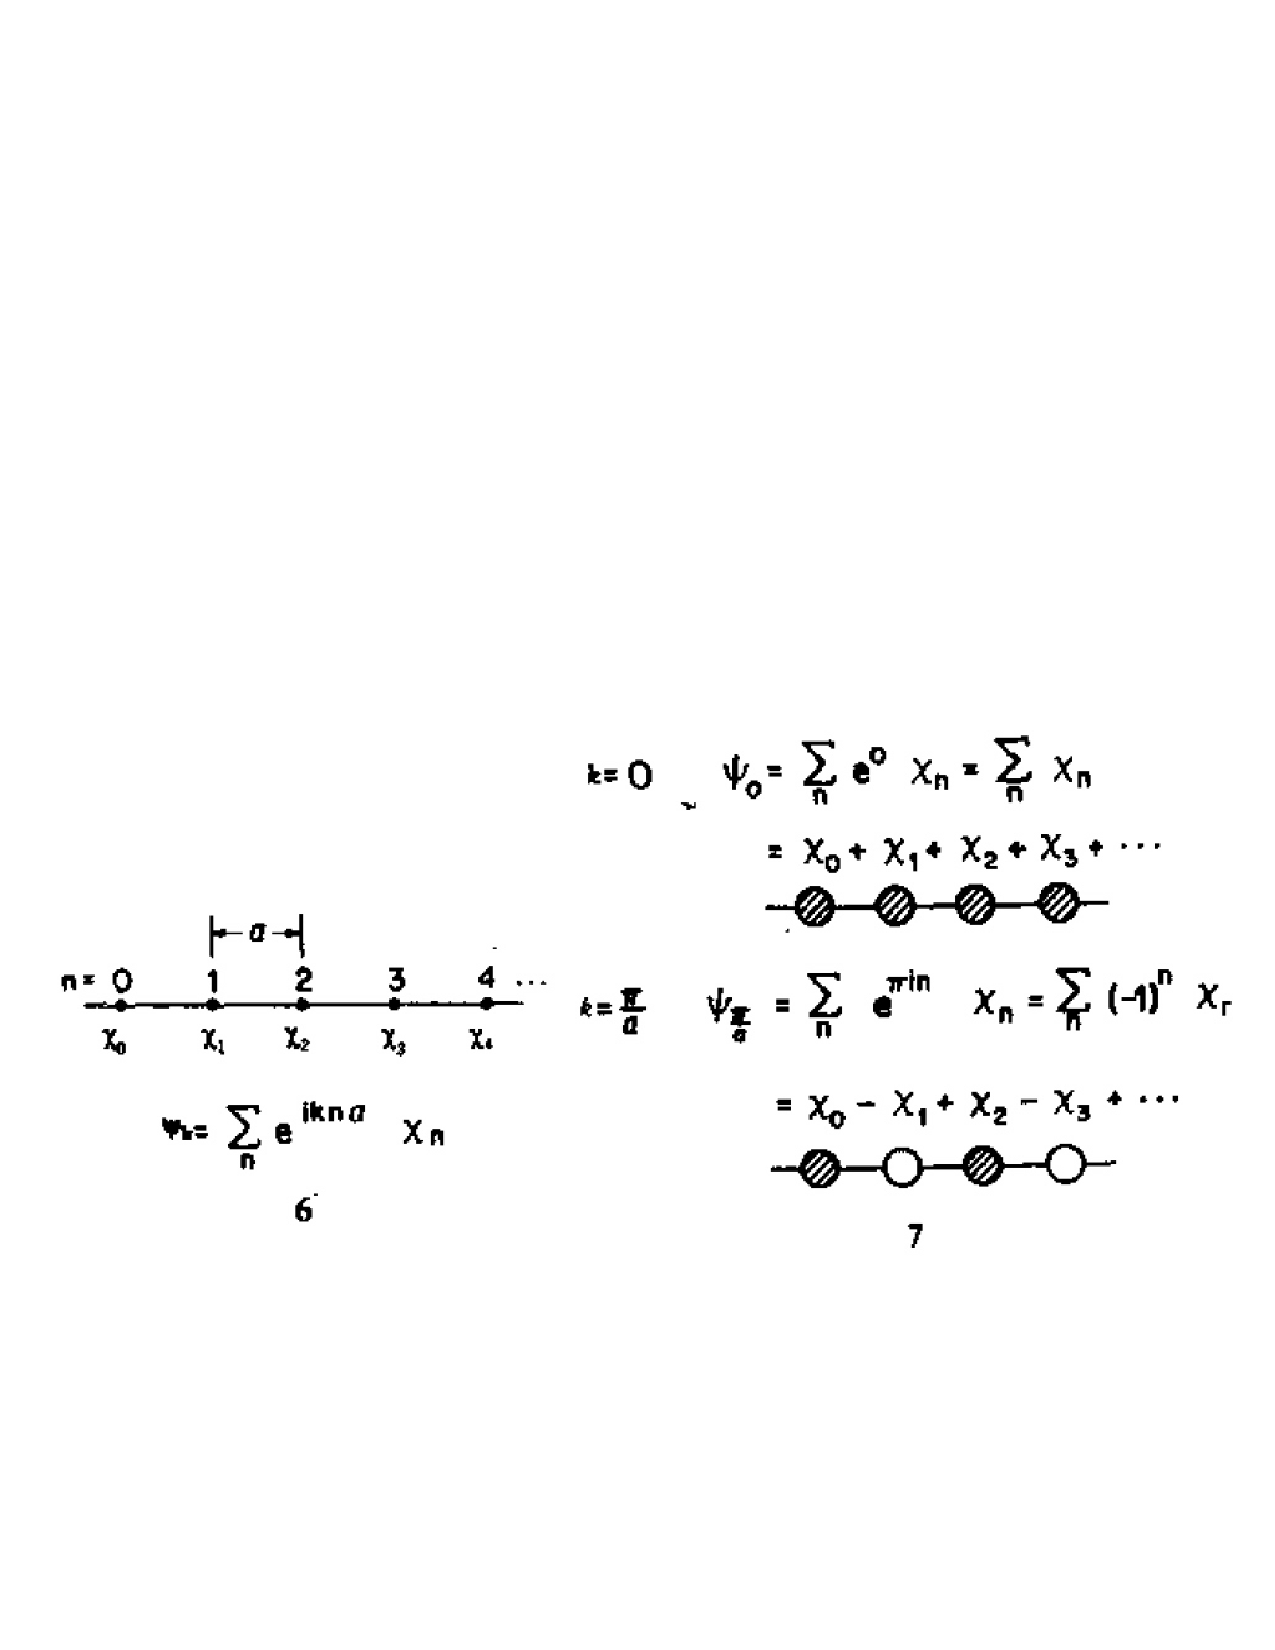
\includegraphics[height=0.5in,width=1.4in,viewport=25 218 595 440,clip]{Figures/Hydrogen-Psi.pdf}}\\
\subfigure[分子轨道与能带]{
\label{fig:Hydrogen-Band-1D}
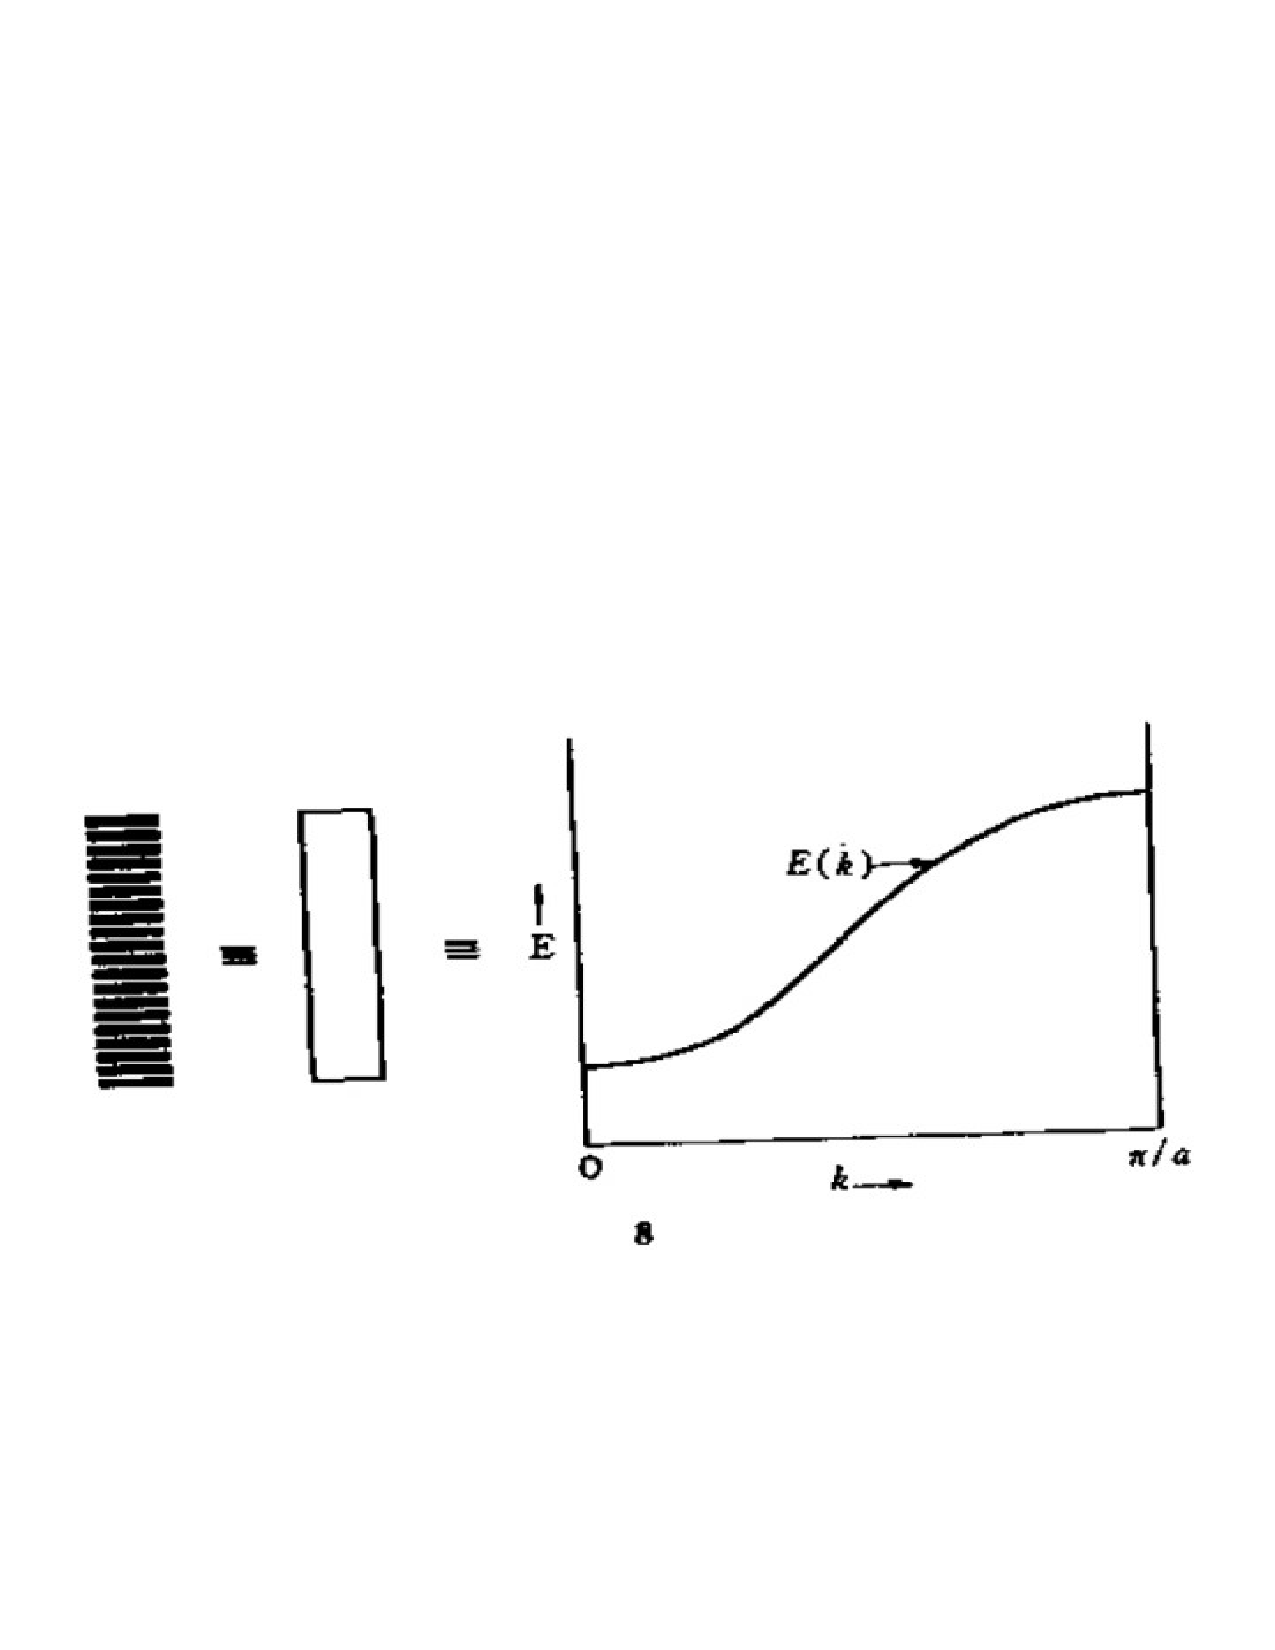
\includegraphics[height=0.6in,width=1.4in,viewport=35 215 575 450,clip]{Figures/Hydrogen-Band-1D.pdf}}
\subfigure[$d$\,轨道]{
\label{fig:Hydrogen-d-Band-1D}
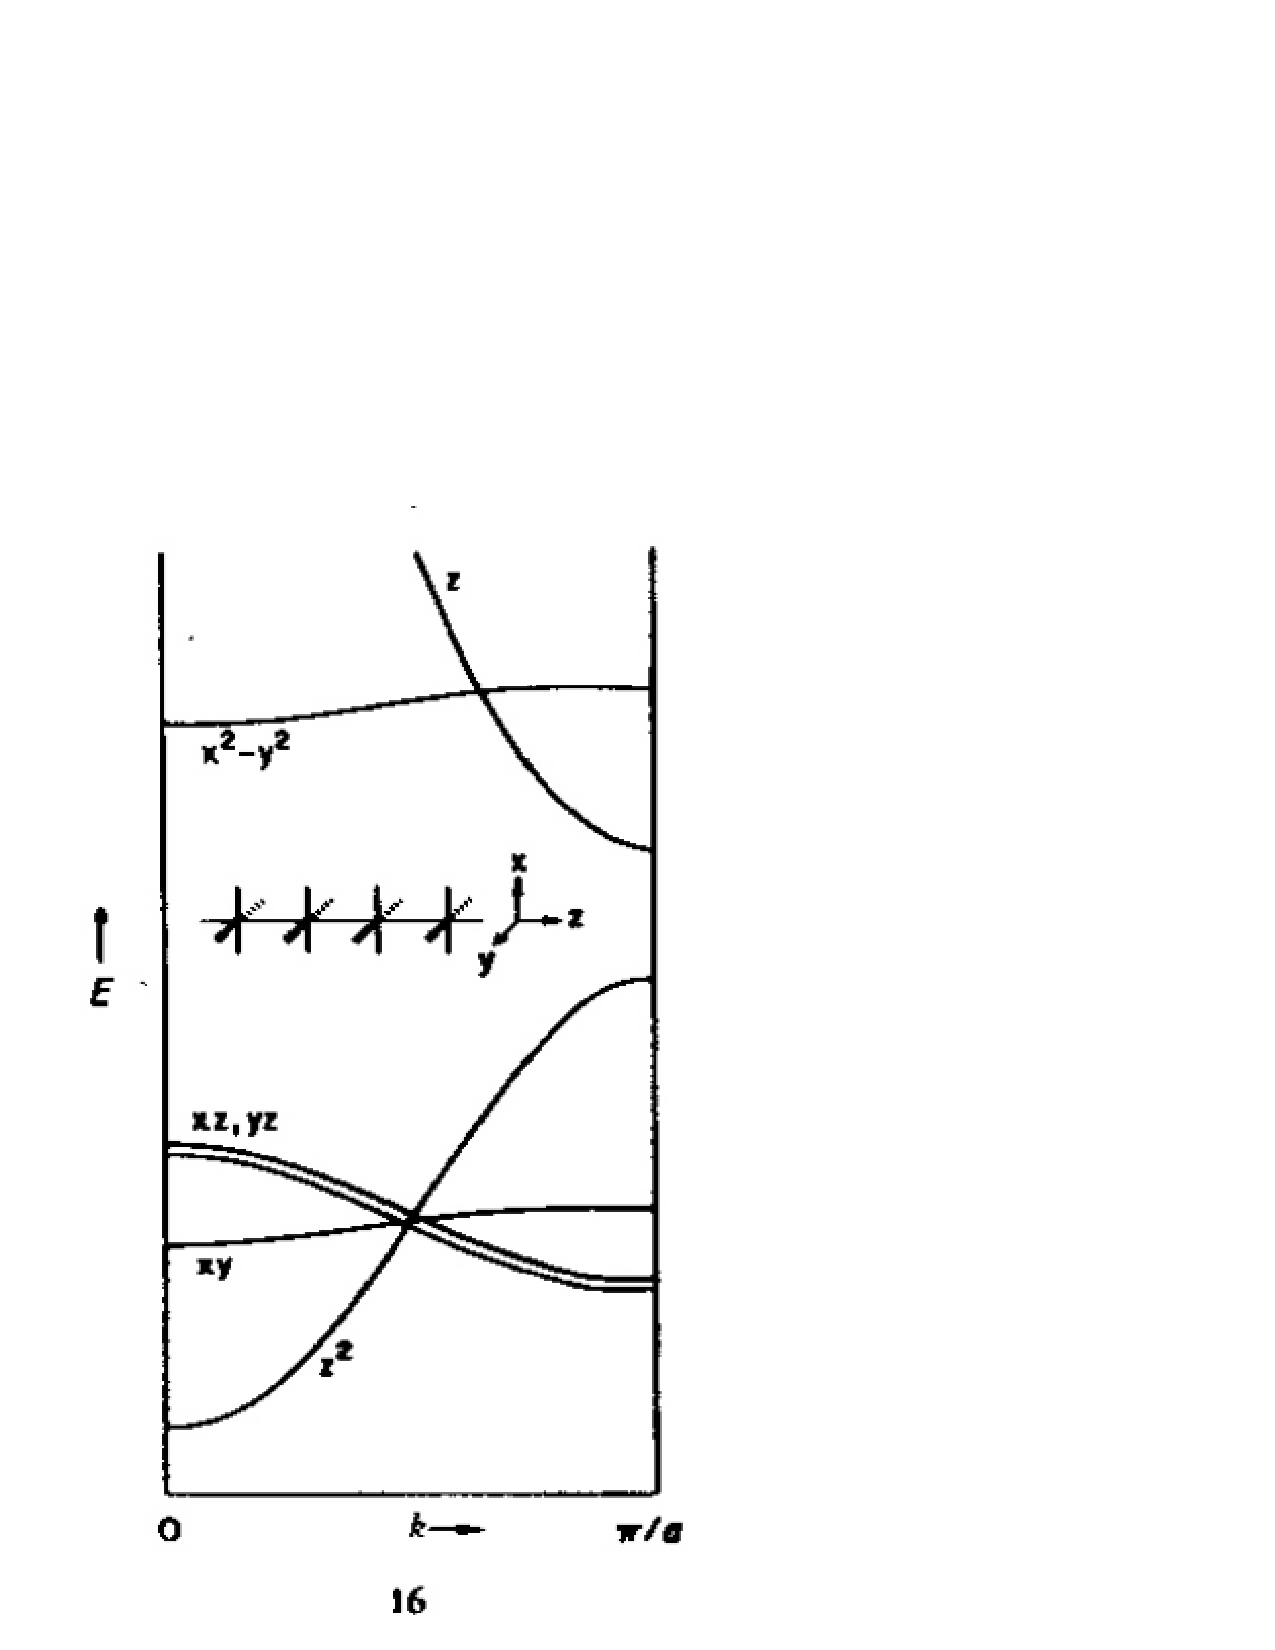
\includegraphics[height=1.0in,width=0.7in,viewport=40 45 330 535,clip]{Figures/Hydrogen-d-Band-1D.pdf}}
\caption{\small \textrm{The Band-structure from Molecular-orbital.}}%
\label{Band-Structure-1}
\end{figure} 
}

\frame
{
\frametitle{周期体系的波函数}
物质的电子体系,可分为芯层分子和价层电子。芯电子能量低,受周围化学环境影响很小,基本保持原子属性;价层电子相互作用较强,对化学环境较为敏感。一般地,价电子波函数在原子间区域(\textrm{Interstitial}区)的变化平缓,在临近原子核附近区域(\textrm{Muffin-tin}球内),会出现剧烈振荡(与芯层波函数正交)。
\begin{figure}[h!]
\centering
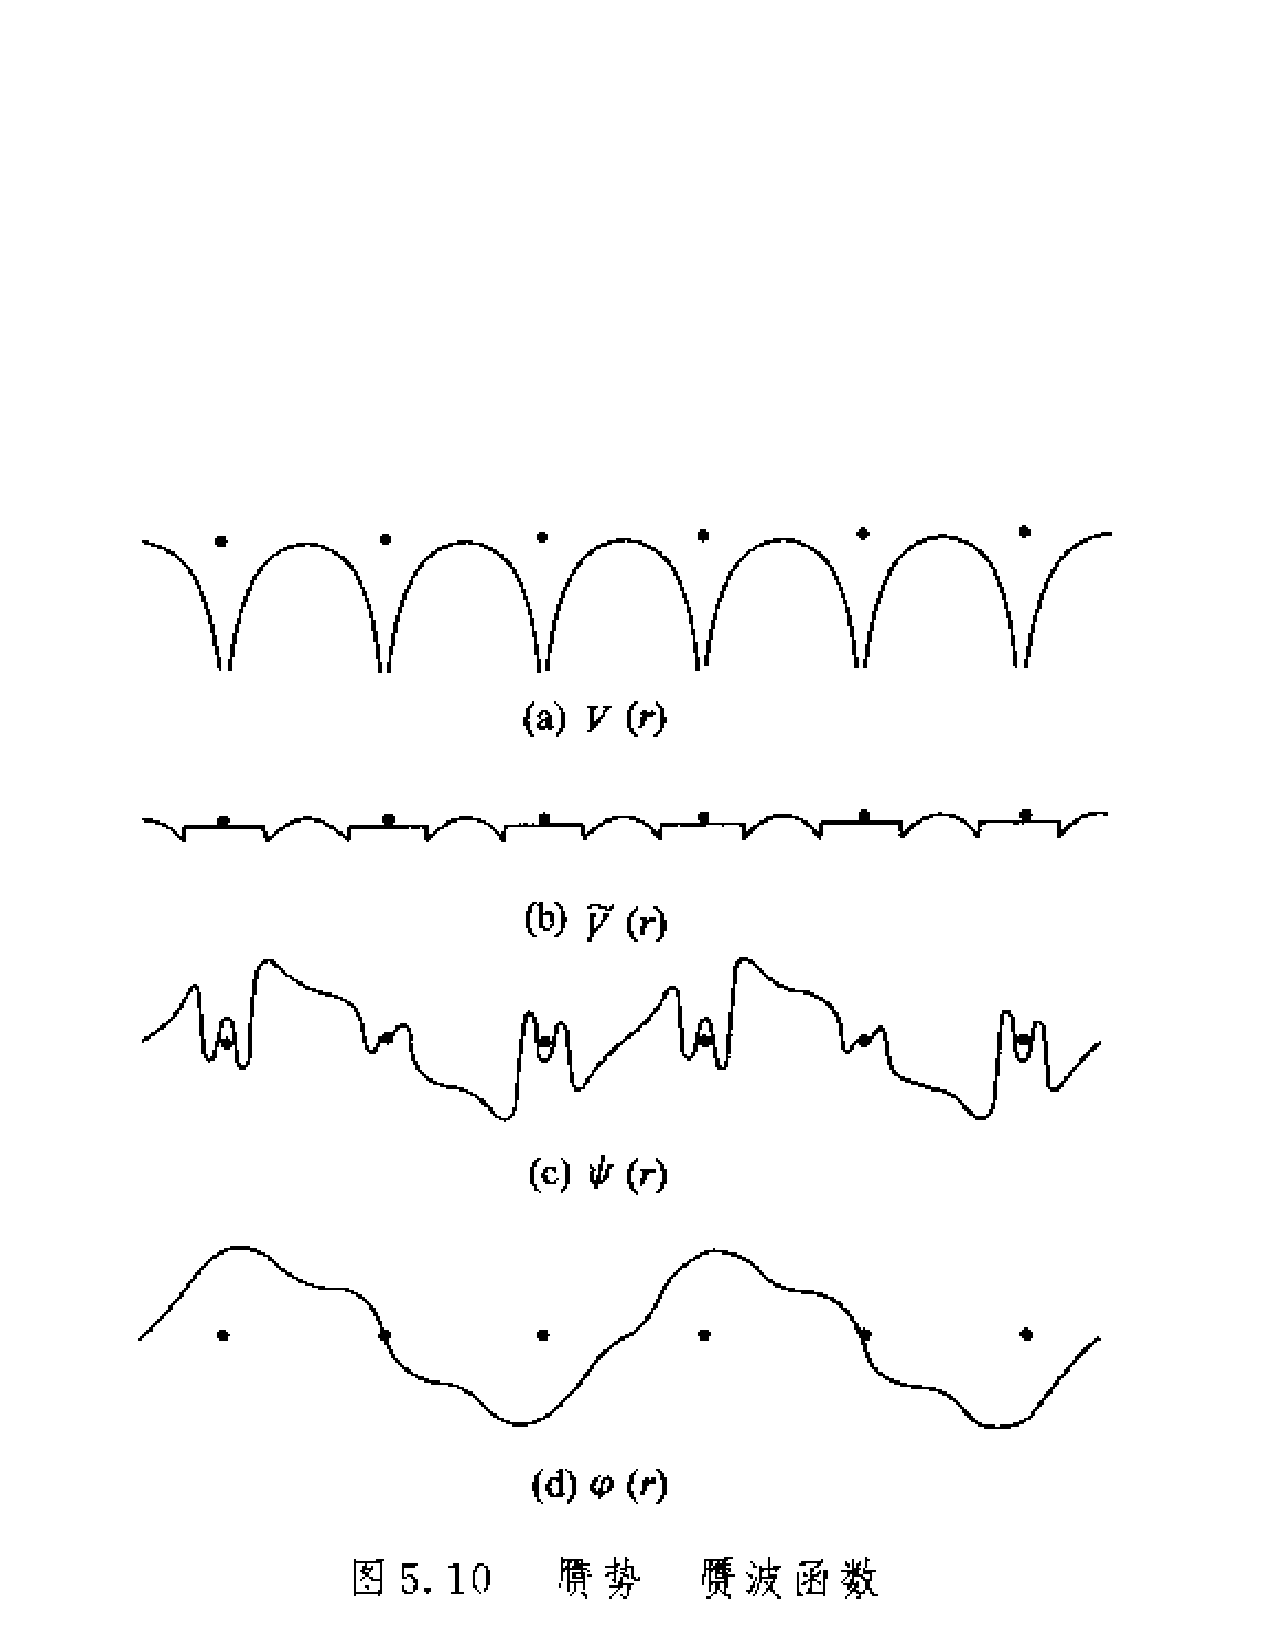
\includegraphics[height=0.8in,width=4.in,viewport=41 433 539 546,clip]{Figures/Pseudo_wave.pdf}\\
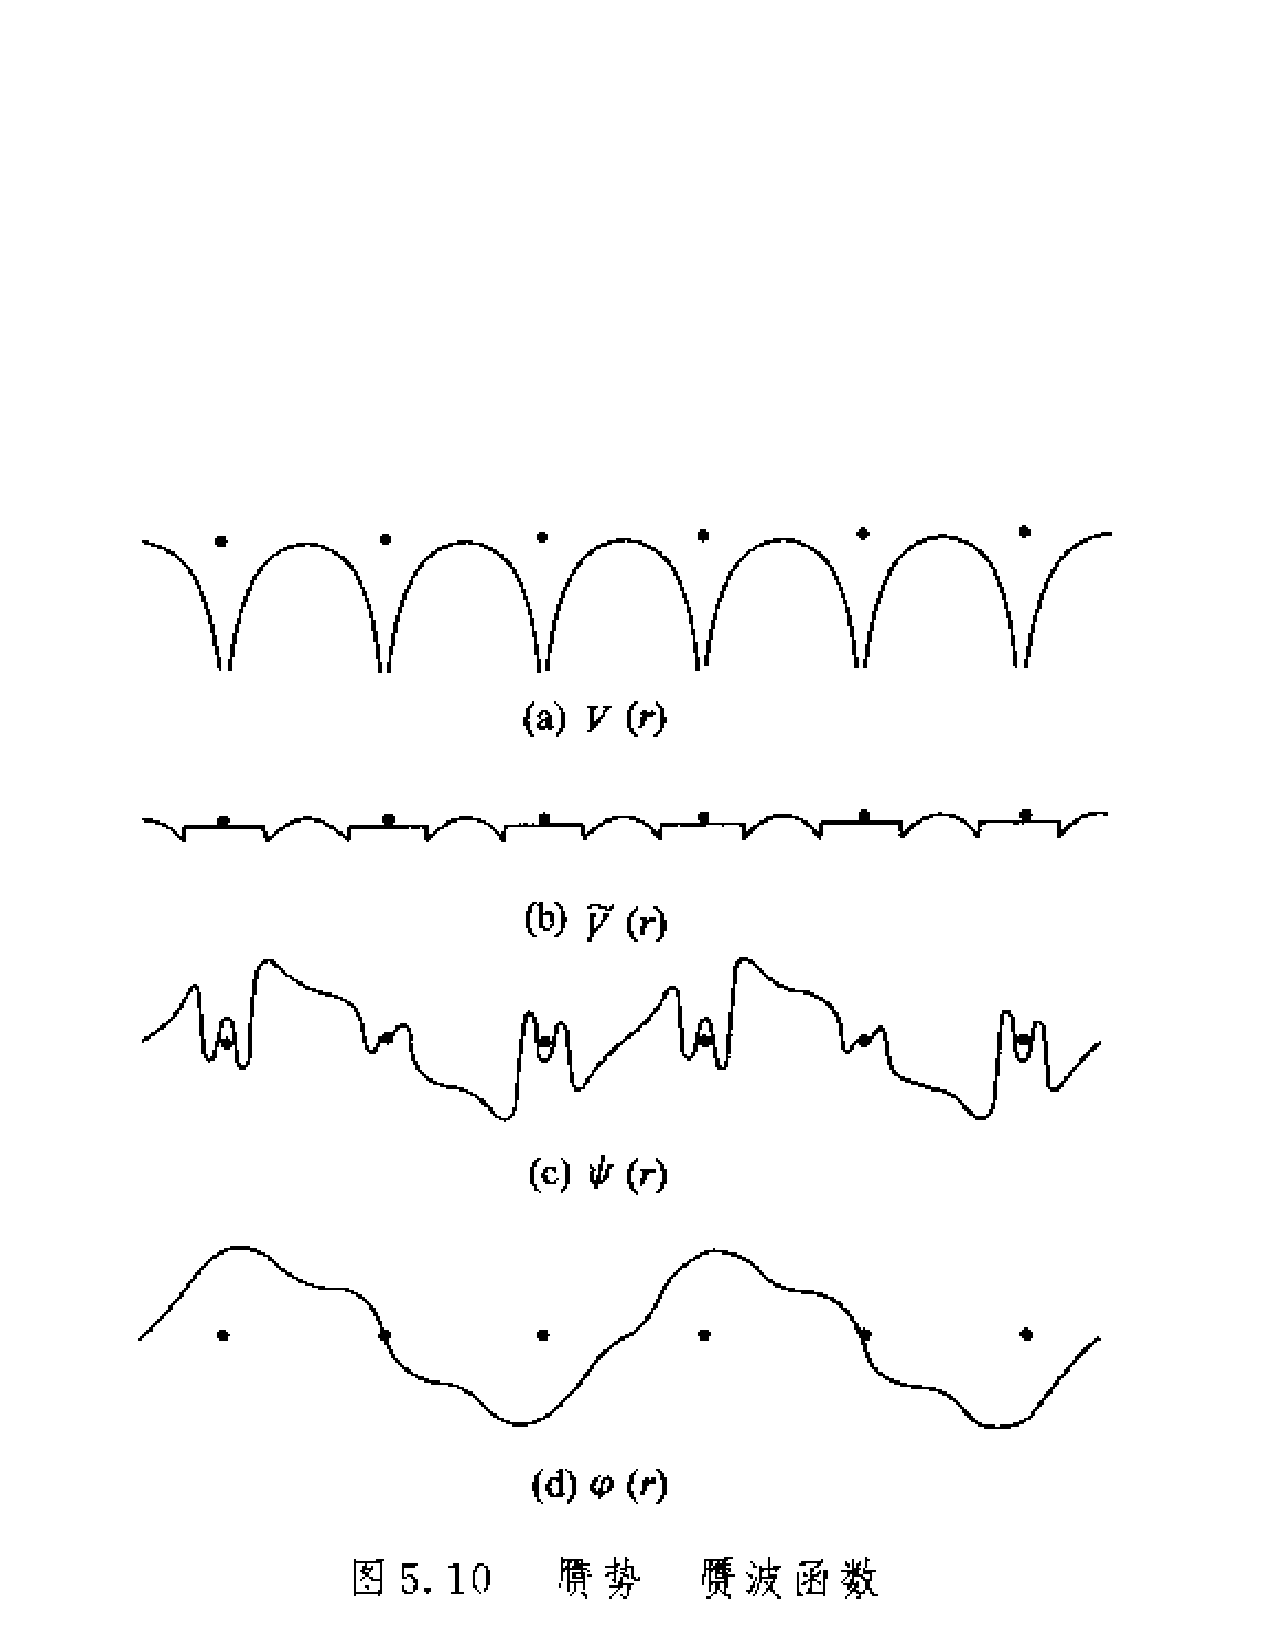
\includegraphics[height=0.8in,width=4.in,viewport=41 210 539 339,clip]{Figures/Pseudo_wave.pdf}
\caption{\small \textrm{The periodic Potential and the wave functions in crystal.}}%(与文献\cite{EPJB33-47_2003}图1对比)
\label{Potential-Wave}
\end{figure}
}

\frame
{
%\frametitle{The methods on band structure calculation}
\frametitle{固体能带计算方法}
%\vskip 10pt
%\textrm{The mainly difference of all these methods below: the basis sets and the construction of the potential}
\vskip 10pt
常用的计算方法
\begin{itemize}%[+-| alert@+>]
%\begin{enumerate}%[+-| alert@+>]
\setlength{\itemsep}{15pt}
%  \item \textrm{Plane wave and the pseudo-potential}
	\item	平面波方法
	\item	正交平面波\textrm{(The orthogonalized plane wave, OPW)}和赝势\textrm{(Pseudo-potential, PP)}方法\upcite{Singh_Book,PRB41-7892_1990,JPCM6-8245_1994}
	\item	缀加平面波\textrm{(Augmented plane wave, APW)}方法
	\item	\textrm{MT}轨道\textrm{(Muffin-tin orbitals, MTO)}方法
	\item	投影子缀加波\textrm{(Projector Augmented Wave, PAW)}方法\upcite{PRB50-17953_1994,PRB59-1758_1999}
\end{itemize}
  \vskip 5pt 各种方法的主要区别:所选的基函数类型不同
}

%\frame
%{
%\frametitle{}
%\begin{figure}[h!]
%\centering
%\vspace*{-10pt}
%\includegraphics[height=2.80in,width=1.70in,viewport=60 90 325 500,clip]{WIEN2k_Program_flow.eps}
%\caption{\small \textrm{Program flow in \textbf{WIEN2k}.}}%(与文献\cite{EPJB33-47_2003}图1对比)
%\label{WIEN2k_program_flow}
%\end{figure}
%}

\frame
{
%\frametitle{The methods on band structure calculation}
\frametitle{由OPW到赝势}
%\vskip 10pt
%\textrm{The mainly difference of all these methods below: the basis sets and the construction of the potential}
\begin{itemize}
\setlength{\itemsep}{5pt}
	\item 完全平面波基组,只要少数的平面波基组就可以很好地描述波函数在原子间的行为,近核的电子波函数则需要大量平面波展开。%因此完全平面波基组虽然方便,但求体系本征态对角化的矩阵非常巨大,计算变得异常耗时。
	\item 正交平面波(\textrm{Orthogonalized plane wave, OPW})方法,价电子用与芯层波函数正交的平面波展开,可以减少平面波数目
		\begin{displaymath}
			\phi_{OPW}^{\vec k+\vec G}(\vec r)=\phi_{PW}^{\vec k+\vec G}(\vec r)-\sum_{\alpha,c}\langle\varphi_c|\phi_{PW}^{\vec k+\vec G}\rangle\varphi_c(\vec r)
		\end{displaymath}
		并且势可以表示为$V^{eff}(\vec r)=V(\vec r)+V^R(\vec r)$,其中排斥部分是$$V^R(\vec r)=\sum_{\alpha,c}(\varepsilon_v-\varepsilon_c)|\varphi_c\rangle\langle\varphi_c|$$
\end{itemize}
}

\frame
{
\frametitle{赝势方法}
赝势(\textrm{Pseudo Potential, PP})方法是在正交平面波的基础上发展起来的,构造出平缓的势函数代替核的强吸引作用和芯层电子的排斥作用,用平缓的函数取代波函数近核时的震荡。
\begin{itemize}
\setlength{\itemsep}{5pt}
	\item 赝势-平面波方法,只需要少量平面波可展开赝波函数,大大提升了计算效率;但是赝波函数不能很好地反映与电子近核行为有关的性质。
	\item 赝势的构造并不唯一,考核构造赝势的两大指标:\\“柔软程度”\textrm{(Soft)}与“可移植性”\textrm{(transferability)}
\end{itemize}
\begin{figure}[h!]
\centering
\vspace*{-0.10in}
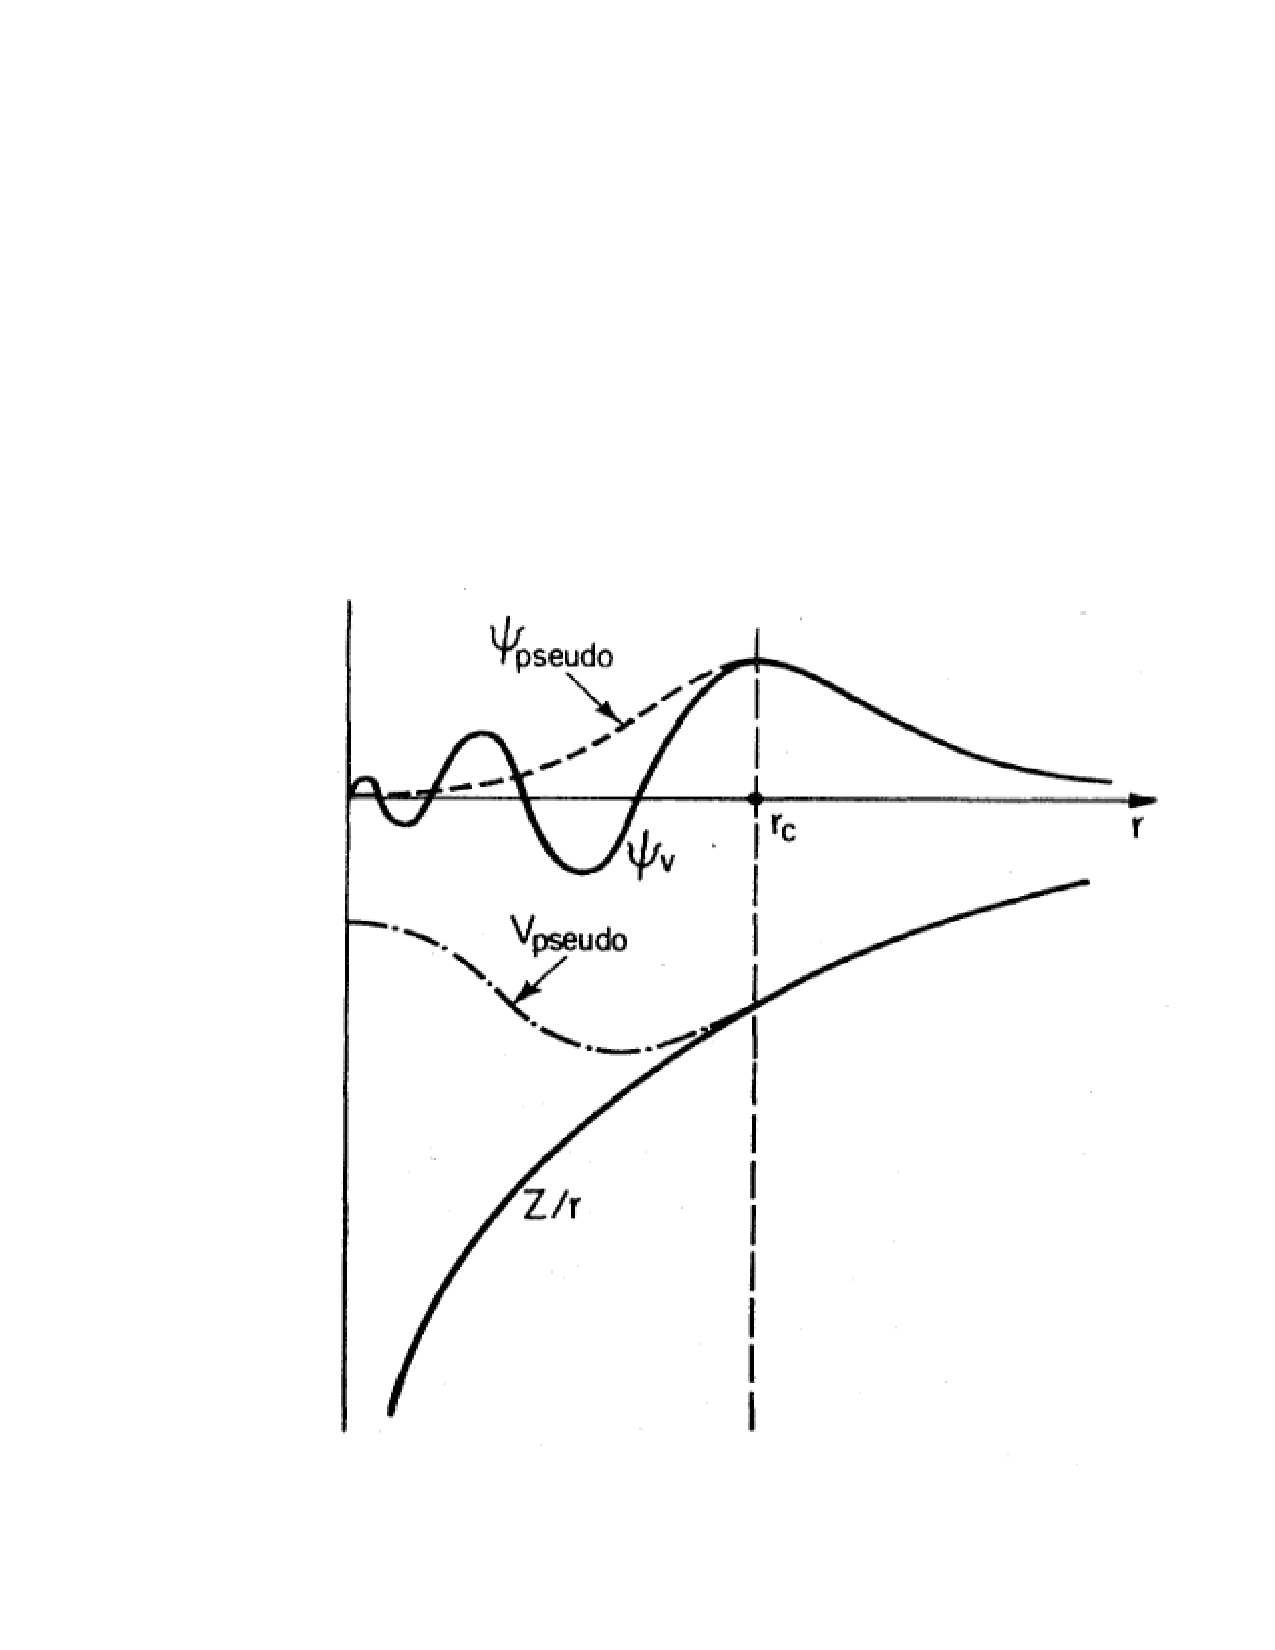
\includegraphics[height=1.35in,width=1.42in,viewport=154 100 562 508,clip]{Figures/Pseudo.pdf}
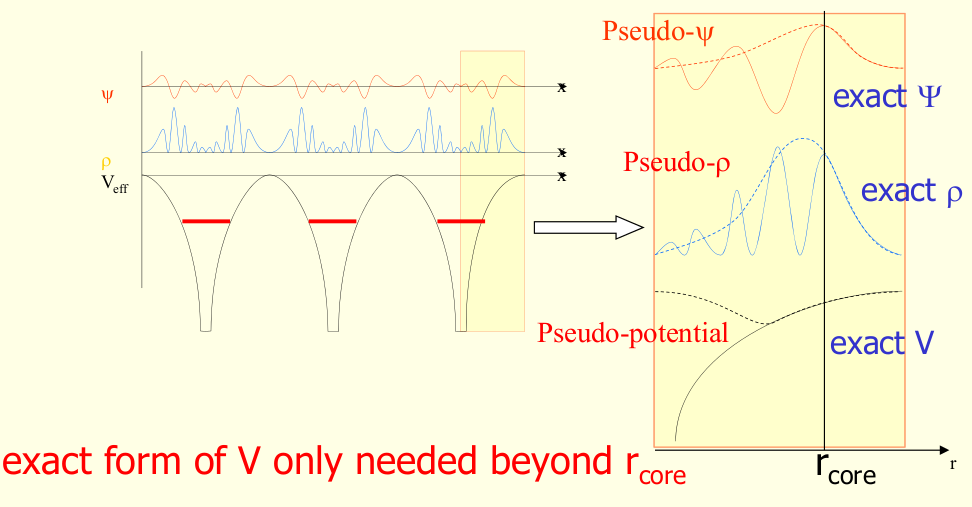
\includegraphics[height=1.35in,width=2.57in,viewport=1 1 980 500,clip]{Figures/Pseudo-2.png}
\caption{\small \textrm{The Pseudo wave function and Pseudo potential.}}%(与文献\cite{EPJB33-47_2003}图1对比)
\label{Pseudo_Potential-Wave}
\end{figure}
}

\frame
{
\frametitle{模守恒赝势和超软赝势}
\begin{itemize}
\setlength{\itemsep}{5pt}
	\item 模守恒\textrm{(Norm-conserving)}赝势,构造赝波函数有约束条件
		\begin{displaymath}
			\int_0^{r_c}\mathrm{d}\vec r\varphi^{\ast PS}(\vec r)\varphi^{PS}(\vec r)=\int_0^{r_c}\mathrm{d}\vec r\varphi^{\ast}(\vec r)\varphi(\vec r)
		\end{displaymath}
	模守恒赝势很好地解决了赝势的可移植性问题
	\item 超软\textrm{(Ultra-soft)}赝势,解除模守恒条件,实现对第一、第二周期元素的高效计算
\end{itemize}
\begin{figure}[h!]
\centering
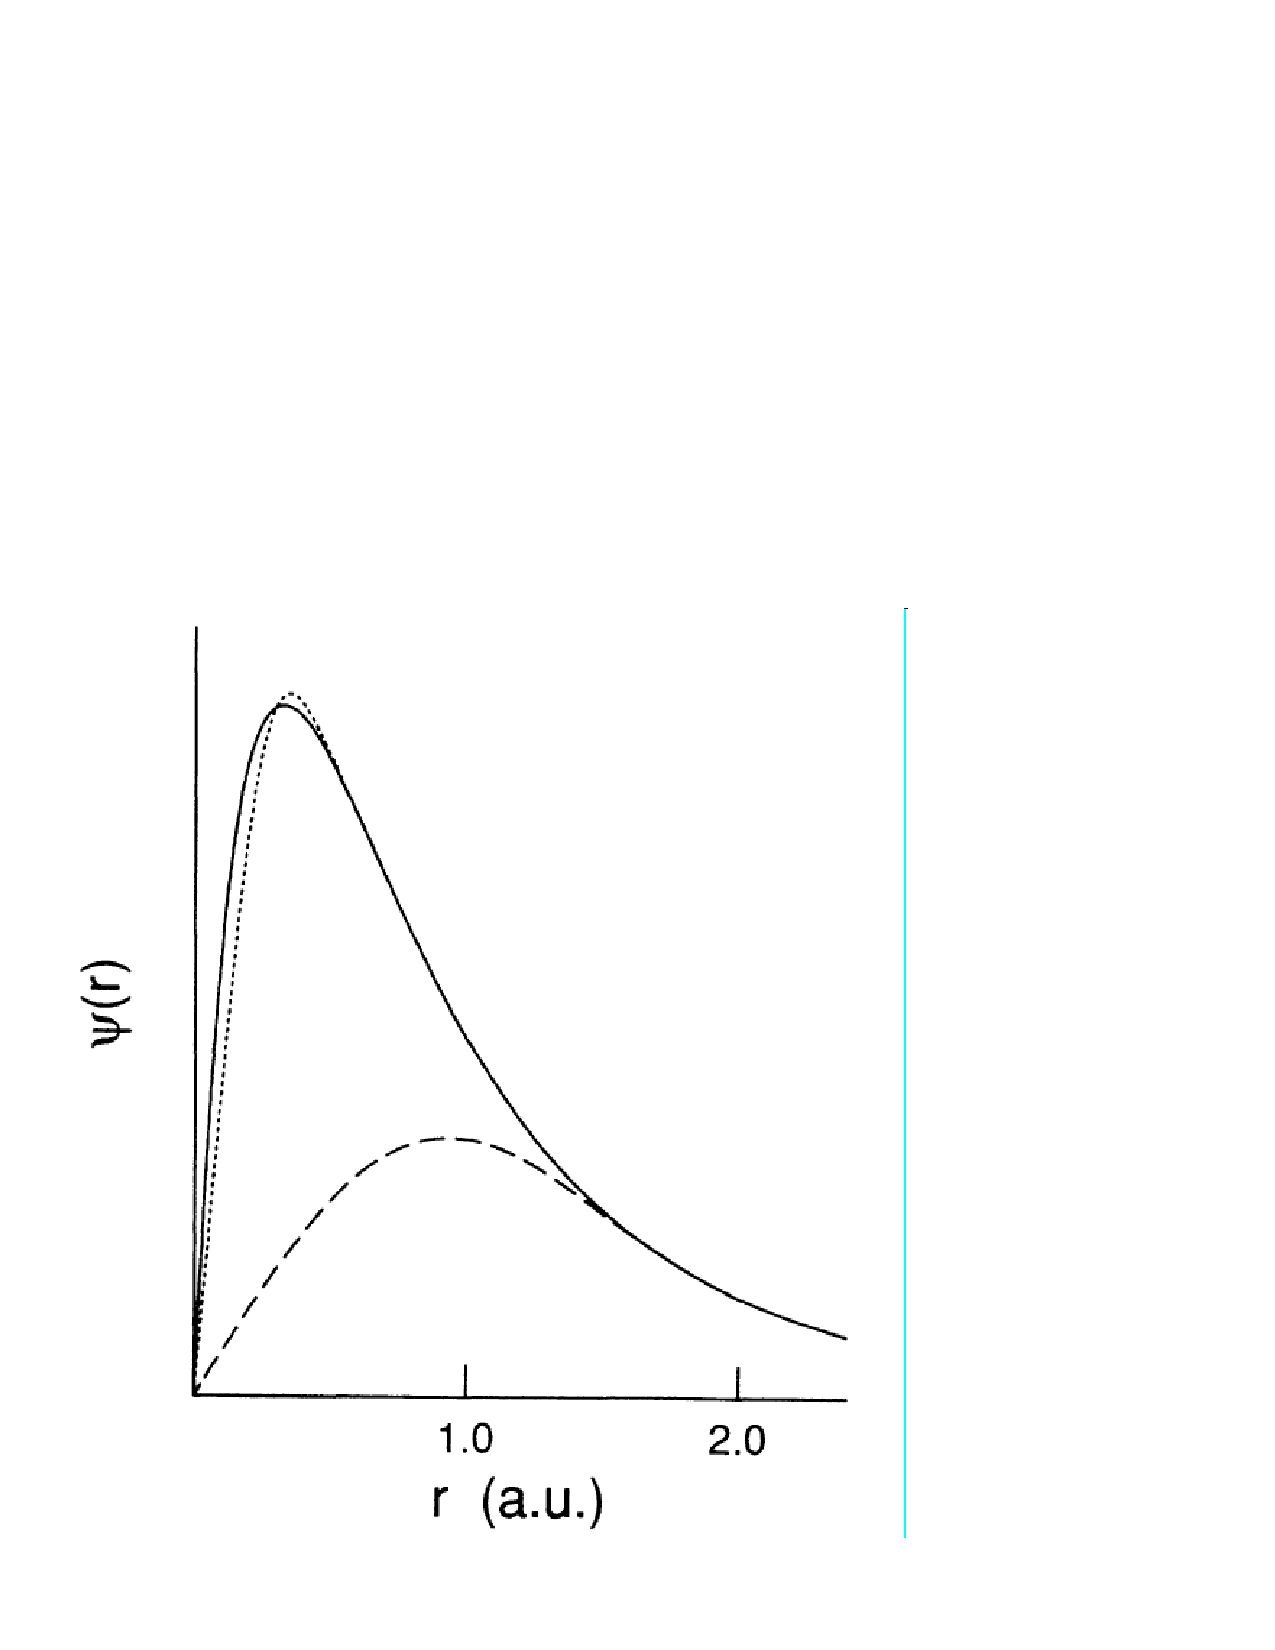
\includegraphics[height=1.35in,width=1.40in,viewport=30 55 415 500,clip]{Figures/Norm-US-wave.pdf}
\caption{\small \textrm{Oxygen 2} \textit{p} \textrm{radical wave function (solid), NC-pseudo-wave (dottde) and US-pseudo-wave (dashed).}}%(与文献\cite{EPJB33-47_2003}图1对比)
\label{Norm-US-wave}
\end{figure}
}

\frame
{
\frametitle{超软赝势}
超软赝势在平缓的局域势函数$V^L(\vec r)$和赝波函数$|\phi_{lmj}(\vec r)\rangle$的基础上,构造函数
\begin{displaymath}
	|\chi_{lmj}(\vec r)\rangle=\bigg[\varepsilon_{lj}-\dfrac12\nabla^2-V^L(\vec r)\bigg]|\phi_{lmj}(\vec r)\rangle
\end{displaymath}
在此基础上得到矩阵$\mathbf{B}_{ij}=\langle\phi_i|\chi_j\rangle$和局域函数
\begin{displaymath}
	|\beta_i\rangle=\sum_j(\mathbf{B}^{-1})_{ji}|\chi_{j}\rangle
\end{displaymath}
因此非局域赝势可以表示为
\begin{displaymath}
	V_{NL}=\dfrac{|\chi_i\rangle\langle\chi_i|}{\langle\chi_i|\chi_i\rangle}=\sum_{i,j}\mathbf{B}_{ij}|\beta_i\rangle\langle\beta_j|
\end{displaymath}
用平缓函数构造赝波函数与真实波函数的电荷密度差
\begin{displaymath}
	Q_{nm}(\vec r)=\varphi_n^{\ast}(\vec r)\varphi_m(\vec r)-\tilde\varphi_n^{\ast}(\vec r)\tilde\varphi_m(\vec r)
\end{displaymath}
}

%\section{微扰公式}       %Bookmark
\section{$\mathrm{PAW}$方法概要}
\frame
{
	\frametitle{\textrm{PAW}方法概要}
\begin{itemize}
	\item 与芯层态正交的全部价电子构成的\textrm{Hilbert}空间%,价电子彼此的正交使得波函数在\textrm{Muffin-tin}球内振荡
	\item 作\textcolor{red}{线性空间变换},全电子波函数$|\Psi\rangle$与赝波函数$|\tilde\Psi\rangle$满足:
		$$|\Psi\rangle=\mathbf{\tau|}\tilde\Psi\rangle$$
%	$$\tau=\mathbf{1}+\sum_{\mathrm R}\hat\tau_{\mathrm R}$$
	\item 在原子核附近的$r_c$范围内,波函数用原子分波函数展开:
	$$|\Psi\rangle=|\tilde\Psi\rangle+\sum_i(|\phi_i\rangle-|\tilde\phi_i\rangle)\langle\tilde p_i|\tilde\Psi\rangle$$
	\item 在$r_c$外$|\tilde\Psi\rangle$与$|\Psi\rangle$变换前后保持不变,因此线性变换$\mathbf{\tau}$可表示为:
	$$\mathbf{\tau}=\mathbf{1}+\sum_i(|\phi_i\rangle-|\tilde\phi_i\rangle)\langle\tilde p_i|$$
\end{itemize}
其中$|\tilde p_i\rangle$是\textrm{MT}球内的投影函数\\
$i$表示原子位置$\vec R$、原子轨道($l,m$)和能级$\epsilon_k$的指标。
}

\frame
{
	\frametitle{\textrm{PAW}方法的基本思想}
	\vspace{10pt}
\begin{figure}[h!]
\centering
\includegraphics[height=1.8in,width=4.in,viewport=30 210 570 440,clip]{Figures/PAW_projector.eps}
\caption{\small \textrm{The analysis of PAW basic function.}}%(与文献\cite{EPJB33-47_2003}图1对比)
\label{PAW_baisc}
\end{figure}
}

\frame
{
\frametitle{\textrm{PAW}方法的基本思想}
	在赝波函数$|\tilde\Psi\rangle$表象下,算符期望值计算满足$$\langle A \rangle=\langle\Psi|\mathbf{A}|\Psi\rangle=\langle\tilde\Psi|\mathbf{\tau}^{\dag}\mathbf{A}\mathbf{\tau}|\tilde\Psi\rangle=\langle\tilde\Psi|\tilde{\mathrm{A}}|\tilde\Psi\rangle$$
\begin{itemize}
	\item 一般赝算符$\tilde A$表示为
		$$\tilde A=\mathbf{A}+\sum_i|\tilde p_i\rangle(\langle\phi_i|\mathbf{A}|\phi_i\rangle-\langle\tilde\phi_i|\mathbf{A}|\tilde\phi_i\rangle)\langle\tilde p_i|$$
	\item 赝重叠算符$\tilde O$表示为
		$$\tilde O=\mathbf{1}+\sum_i|\tilde p_i\rangle(\langle\phi_i|\phi_i\rangle-\langle\tilde\phi_i|\tilde\phi_i\rangle)\langle\tilde p_i|$$
\end{itemize}
}

\frame
{
\frametitle{\textrm{PAW}方法密度计算}
在\textrm{PAW}框架下,将密度算符$|\vec r\rangle\langle\vec r|$代入,可知密度表达式为
$$n(\vec r)=\tilde n(\vec r)+n^1(\vec r)-\tilde n^1(\vec r)$$
这里
$$\tilde n(\vec r)=\sum_nf_n\langle\tilde\Psi_n|\vec r\rangle\langle\vec r|\tilde\Psi_n\rangle$$ 
$$n^1(\vec r)=\sum_{n,(i,j)}f_n\langle\tilde\Psi_n|\tilde p_i\rangle\langle\phi_i|\vec r\rangle\langle\vec r|\phi_j\rangle\langle\tilde p_j|\tilde\Psi_n\rangle$$
$$\tilde n^1(\vec r)=\sum_{n,(i,j)}f_n\langle\tilde\Psi_n|\tilde p_i\rangle\langle\tilde\phi_i|\vec r\rangle\langle\vec r|\tilde\phi_j\rangle\langle\tilde p_j|\tilde\Psi_n\rangle$$
}

\frame
{
\frametitle{\textrm{PAW}方法总能量的计算}
总能量泛函
%\begin{displaymath}
%	\begin{aligned}
%		E&=\sum_nf_n\langle\Psi_n|-\dfrac12\nabla^2|\Psi_n\rangle\\
%		 &+\dfrac12\int\mathrm{d}\vec r\int\mathrm{d}\vec r^{\prime}\dfrac{(n+n^Z)(n+n^Z)}{|\vec r-\vec r^{\prime}|}+\int\mathrm{d}\vec r n\epsilon_{\mathrm{XC}}(n)
%	\end{aligned}
%\end{displaymath}
$E=\tilde E+E^1-\tilde E^1$,每一项分别表示为:
\begin{displaymath}
	\begin{aligned}
		\tilde E&=\sum_nf_n\langle\tilde\Psi_n|-\dfrac12\nabla^2|\tilde\Psi_n\rangle\\
		 &+\dfrac12\int\mathrm{d}\vec r\int\mathrm{d}\vec r^{\prime}\dfrac{(\tilde n+\hat n)(\tilde n+\hat n)}{|\vec r-\vec r^{\prime}|}+\int\mathrm{d}\vec r \tilde n\bar v+\int\mathrm{d}\vec r \tilde n\epsilon_{\mathrm{XC}}(\tilde n)
 	\end{aligned}
\end{displaymath}
\begin{displaymath}
	\begin{aligned}
		E^1&=\sum_{n,(i,j)}f_n\langle\tilde\Psi_n|\tilde p_i\rangle\langle\phi_i|-\dfrac12\nabla^2|\phi_j\rangle\langle\tilde p_j|\tilde\Psi_n\rangle\\
		 &+\dfrac12\int\mathrm{d}\vec r\int\mathrm{d}\vec r^{\prime}\dfrac{(n^1+n^Z)(n^1+n^Z)}{|\vec r-\vec r^{\prime}|}+\int\mathrm{d}\vec r n^1\epsilon_{\mathrm{XC}}(n^1)
 	\end{aligned}
\end{displaymath}
\begin{displaymath}
	\begin{aligned}
		\tilde E^1&=\sum_{n,(i,j)}f_n\langle\tilde\Psi_n|\tilde p_i\rangle\langle\tilde\phi_i|-\dfrac12\nabla^2|\tilde\phi_j\rangle\langle\tilde p_j|\tilde\Psi_n\rangle\\
		 &+\dfrac12\int\mathrm{d}\vec r\int\mathrm{d}\vec r^{\prime}\dfrac{(\tilde n^1+\hat n)(\tilde n^1+\hat n)}{|\vec r-\vec r^{\prime}|}+\int\mathrm{d}\vec r \tilde n^1\bar v+\int\mathrm{d}\vec r \tilde n^1\epsilon_{\mathrm{XC}}(\tilde n^1)
 	\end{aligned}
\end{displaymath}
}

\frame
{
	\frametitle{\textrm{PAW}原子数据集}
\textrm{PAW}原子数据集是在原子核附近$r_c$范围内将波函数用原子分波展开所需信息的统称,是\textrm{PAW}计算的基础。

\textrm{PAW}原子数据集主要包括
	\begin{itemize}
		\item 分波信息:原子分波$\phi_i$、赝分波$\tilde\phi_i$和投影子波函数$p_i$
		\item 密度信息:$r_c$内的电荷密度$n^1$、赝电荷密度$\tilde n^1$和补充电荷$\hat n$
		\item 赝势信息:局域赝势$\tilde v_{loc}(\vec r)$
	\end{itemize}
	与赝势方法相似,一套原子数据集将用于各种化学环境下的\textrm{PAW}计算,即要求原子数据集有良好的可移植性;与赝势方法不同之处在于\textrm{PAW}原子集中除了赝原子的信息,还包含了真实原子的信息。
}

\section{$\vec k$空间积分与布点}
\frame
{
\frametitle{能带、\textrm{Fermi}面与$\vec k$空间积分}
\vspace{30pt}
\begin{figure}[h!]
\centering
\hspace*{-0.30in}
\subfigure[\textrm{Band structure}]{
\label{Band_Gap_Fermi-1}
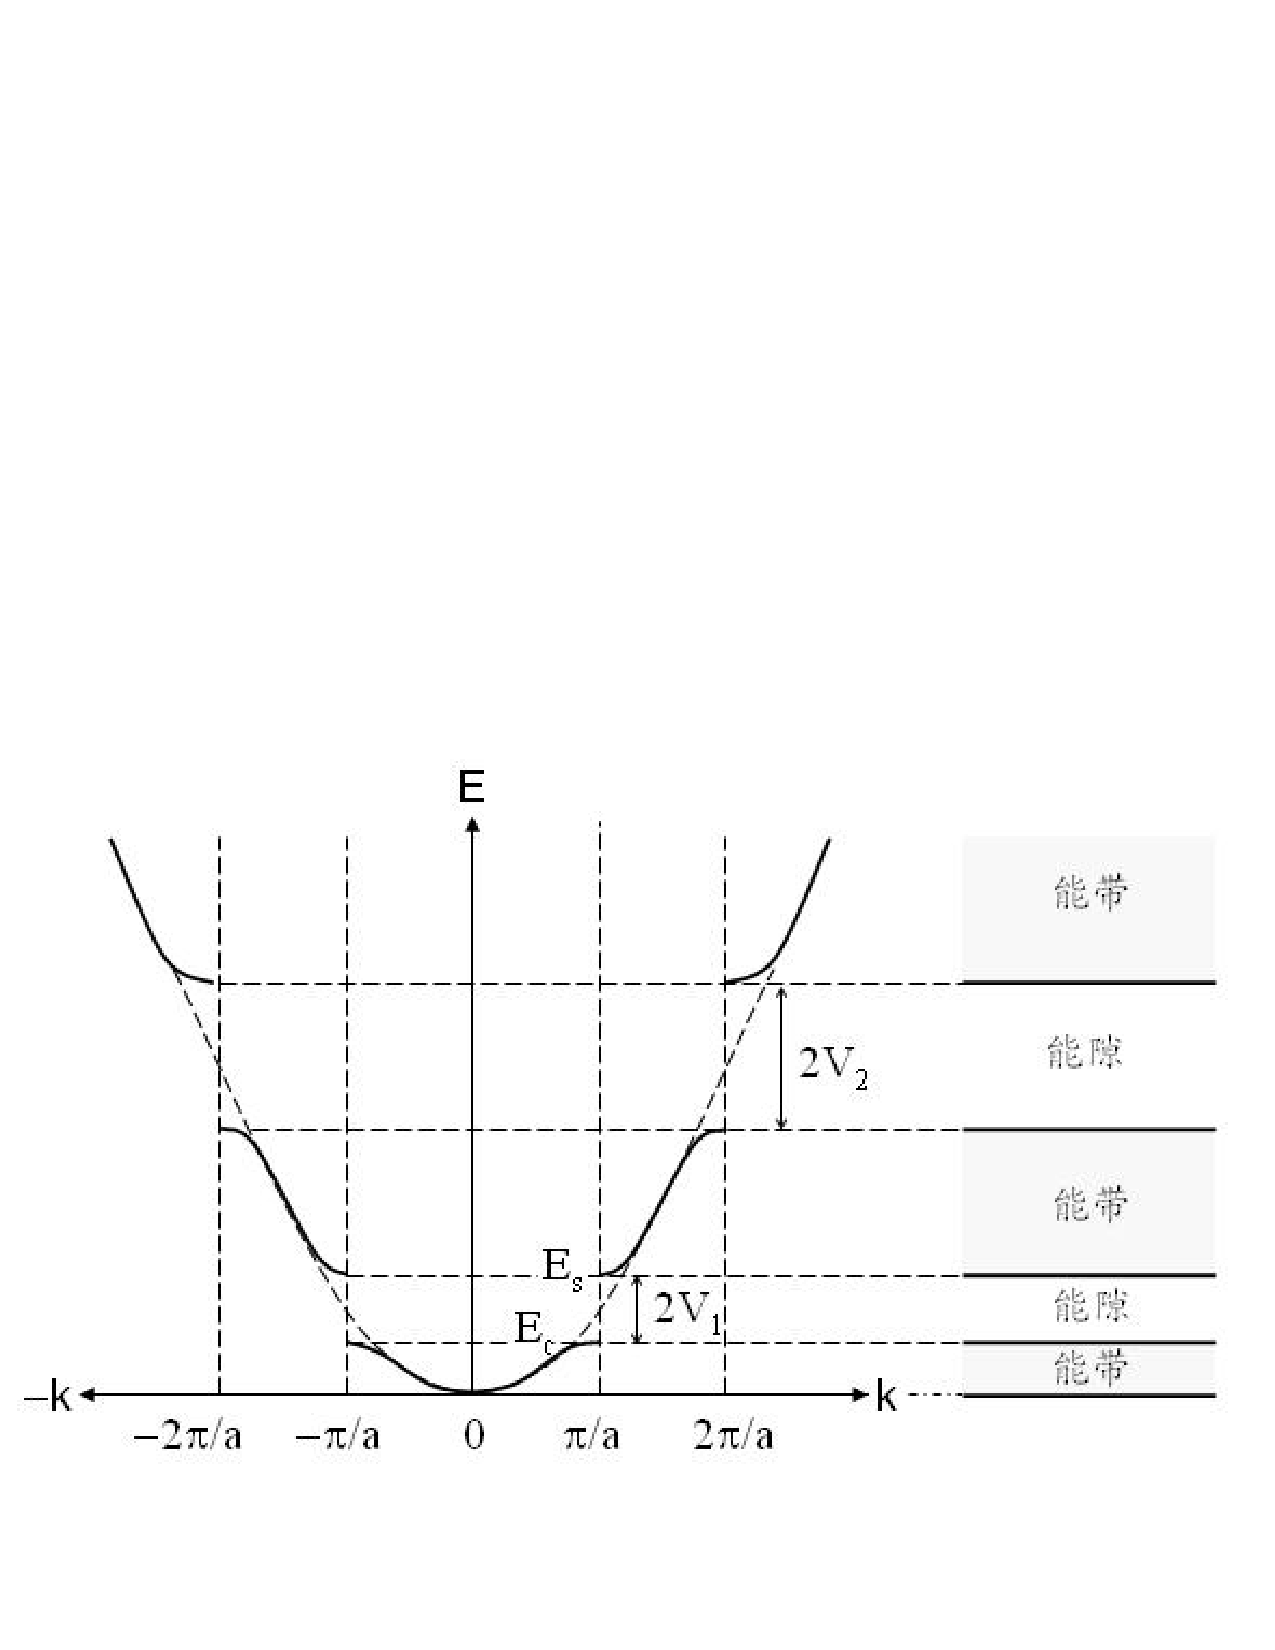
\includegraphics[height=1.3in,width=2.3in,viewport=10 90 570 380,clip]{Figures/Band_Gap.pdf}}
\subfigure[\textrm{Brillouin Zone}]{
\label{Band_Gap_Fermi-2}
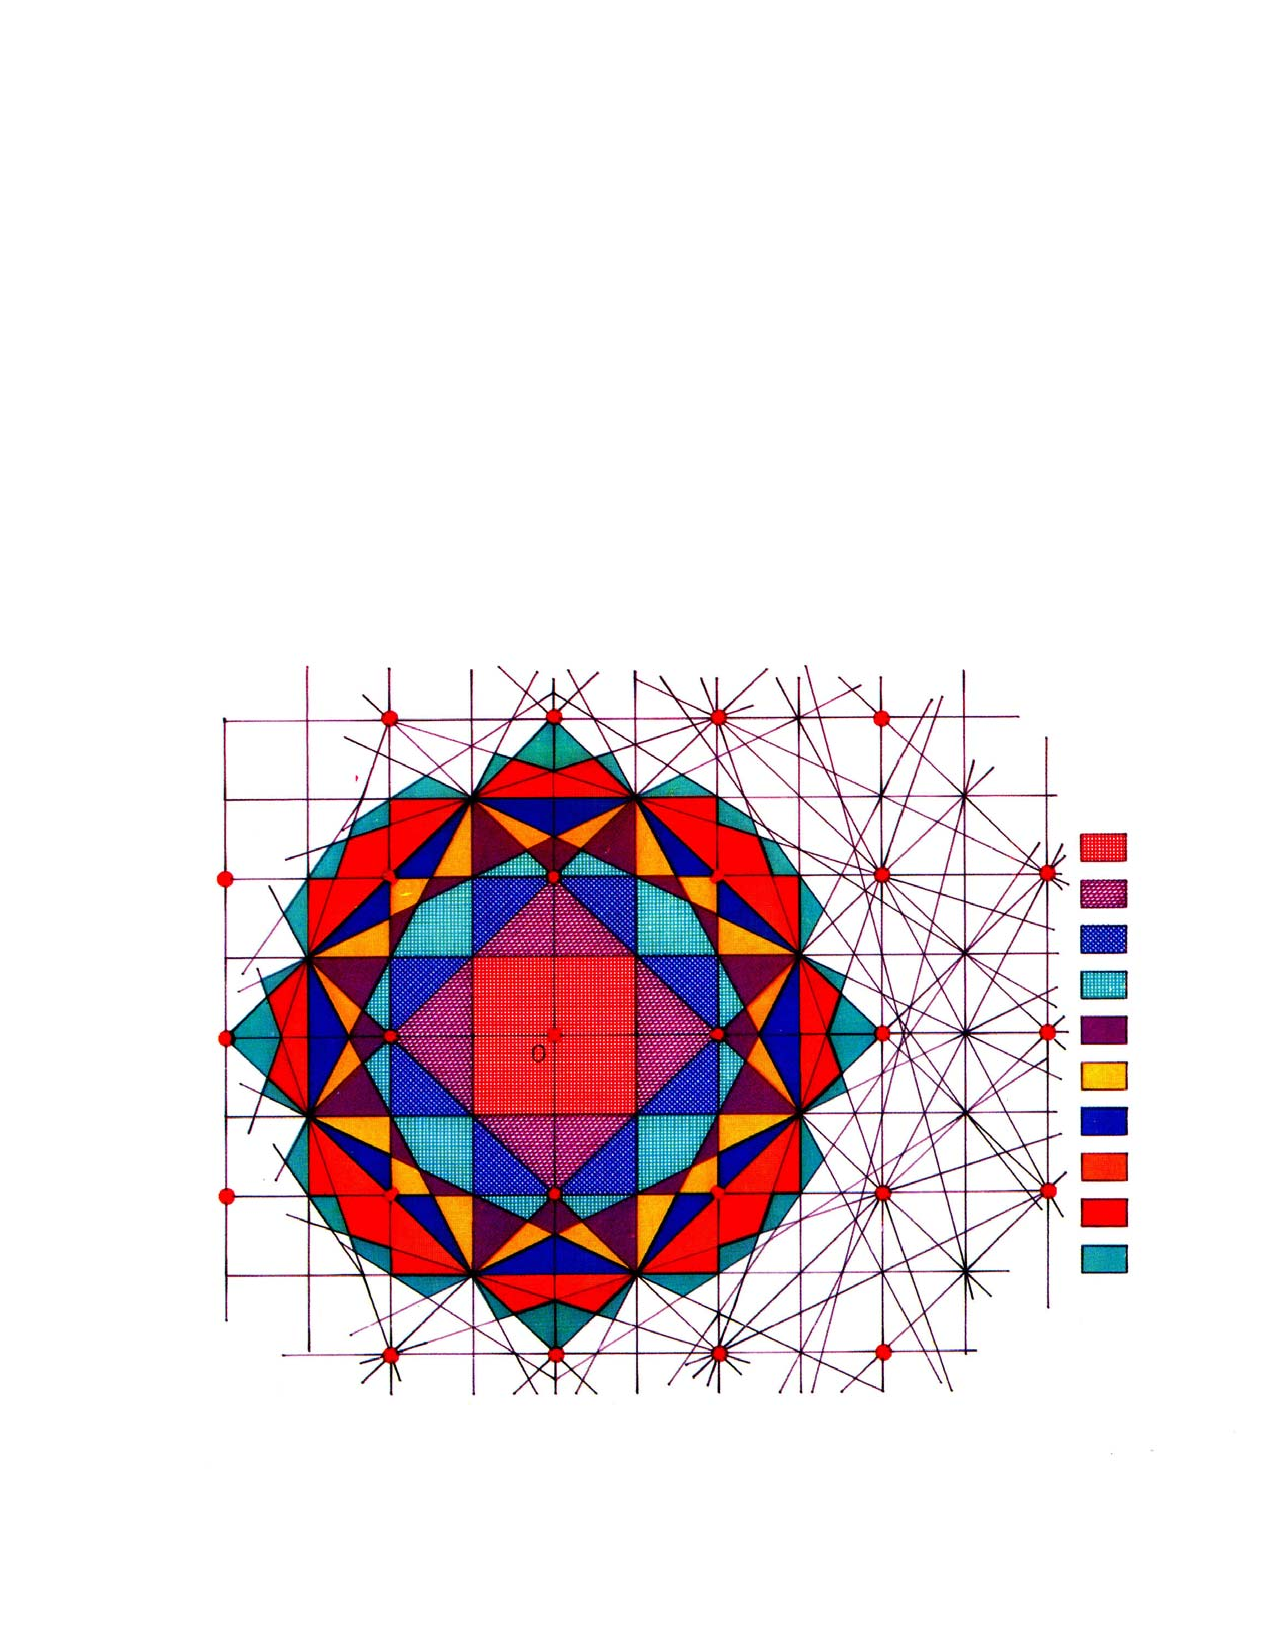
\includegraphics[height=1.28in,width=1.75in,viewport=100 120 545 470,clip]{Figures/2D_Brillouin-Zone.pdf}}
\label{Band_Gap_Fermi}
\end{figure}
}

\frame
{
\frametitle{$\vec k$ 空间布点方案}
\vskip 10pt
周期性体系计算,涉及除了在每个格点上求解\textrm{Schr\"odinger}方程外,计算固体性质的时还需要对$\vec k$空间中完成数值积分。
%\textbf{期望值},$\vec k$空间布点数值测试
\vskip 5pt
\begin{itemize}%[+-| alert@+>]
%\begin{enumerate}%[+-| alert@+>]
%\item $\vec k$空间布点方案
%  \begin{enumerate}
%\setlength{\itemsep}{15pt}
    \item 特殊点布点方案\textrm{(spectial points method)}\\
      将\textrm{Brillouin}区的积分变成网格点的权重求和
    \item 四面体布点方案\textrm{(tetrahedron method)}\upcite{PRB49-16233_1994}\\
	    \textrm{Brillouin}区积分转换为对网格点构成的四面体求和
%  \end{enumerate}
\end{itemize}
\begin{figure}[h!]
\centering
\vspace*{-0.2in}
\subfigure[\textrm{Special points}]{
\label{Special_Points-1}
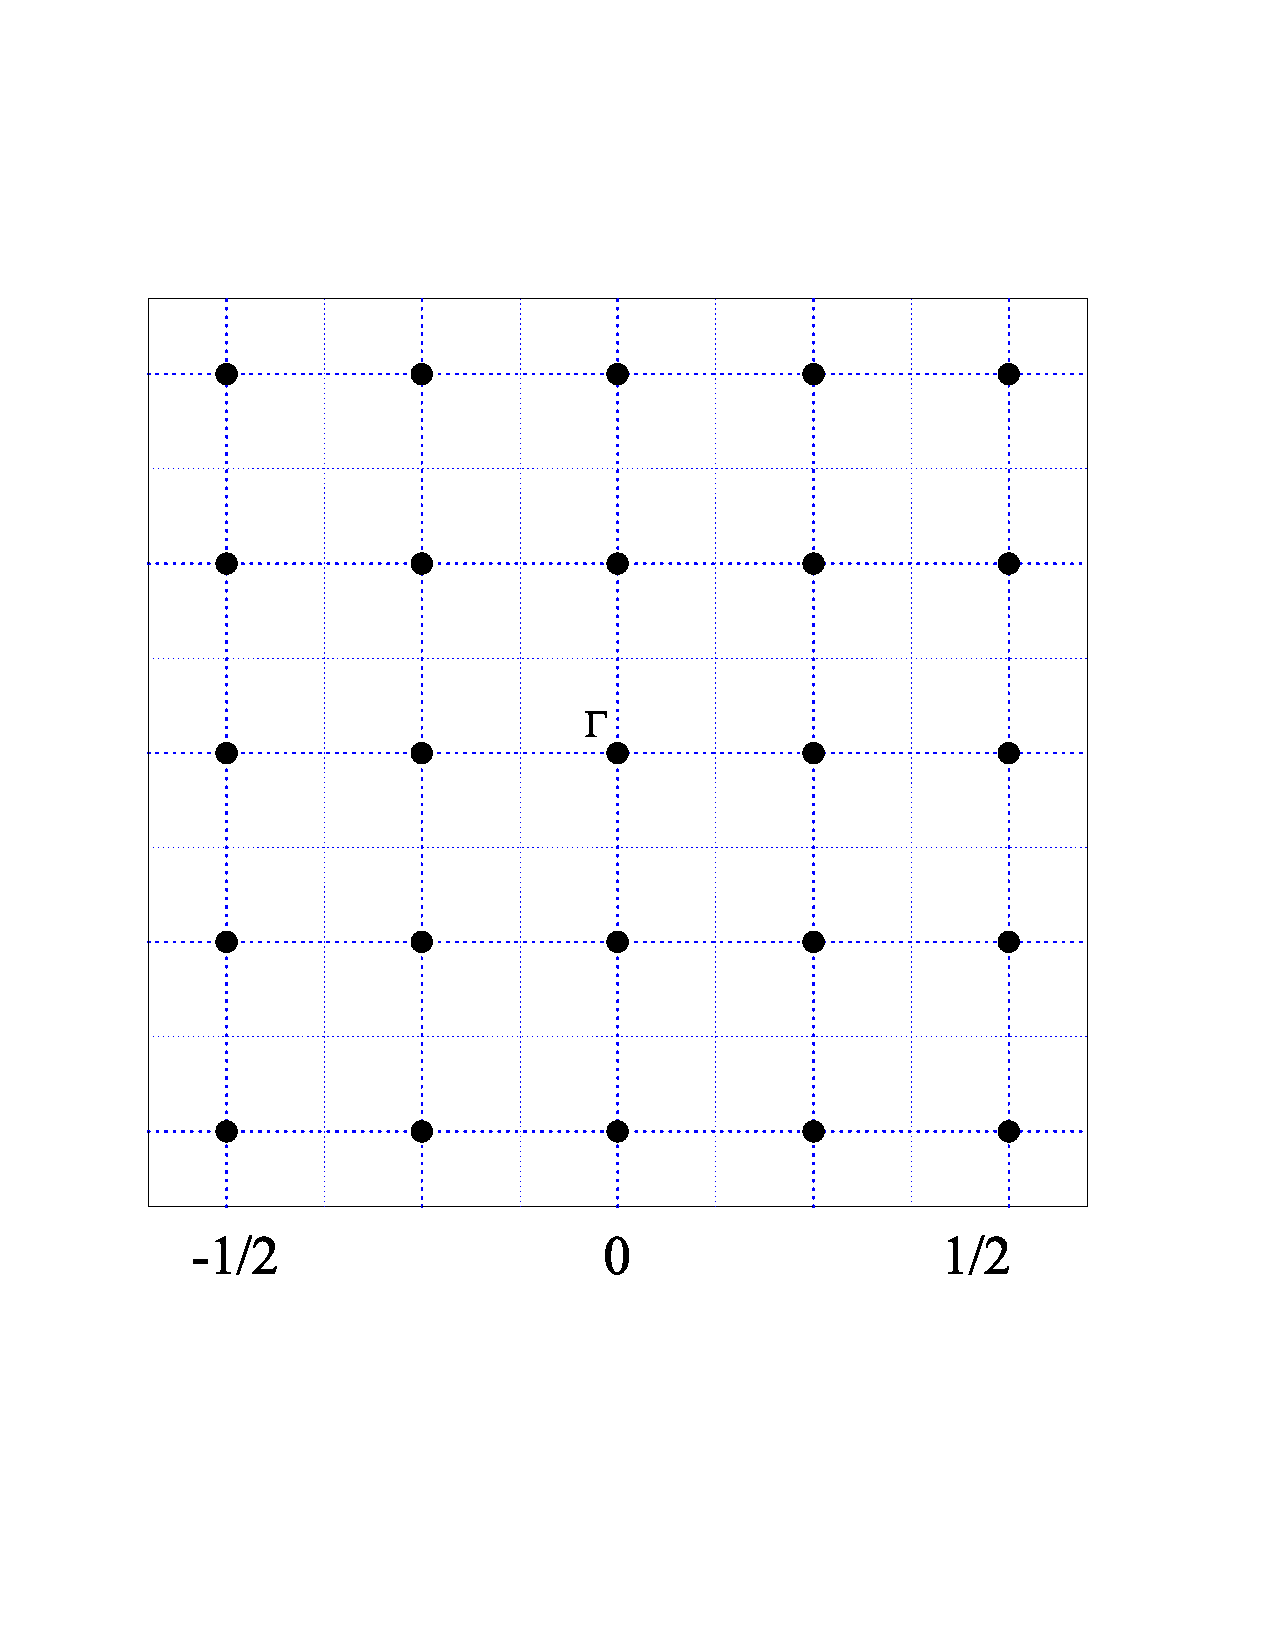
\includegraphics[height=1.28in,width=1.24in,viewport=65 175 525 650,clip]{Figures/Special-points-1.pdf}}
\subfigure[\textrm{Tetrahedron}]{
\label{Tetrahedron-2}
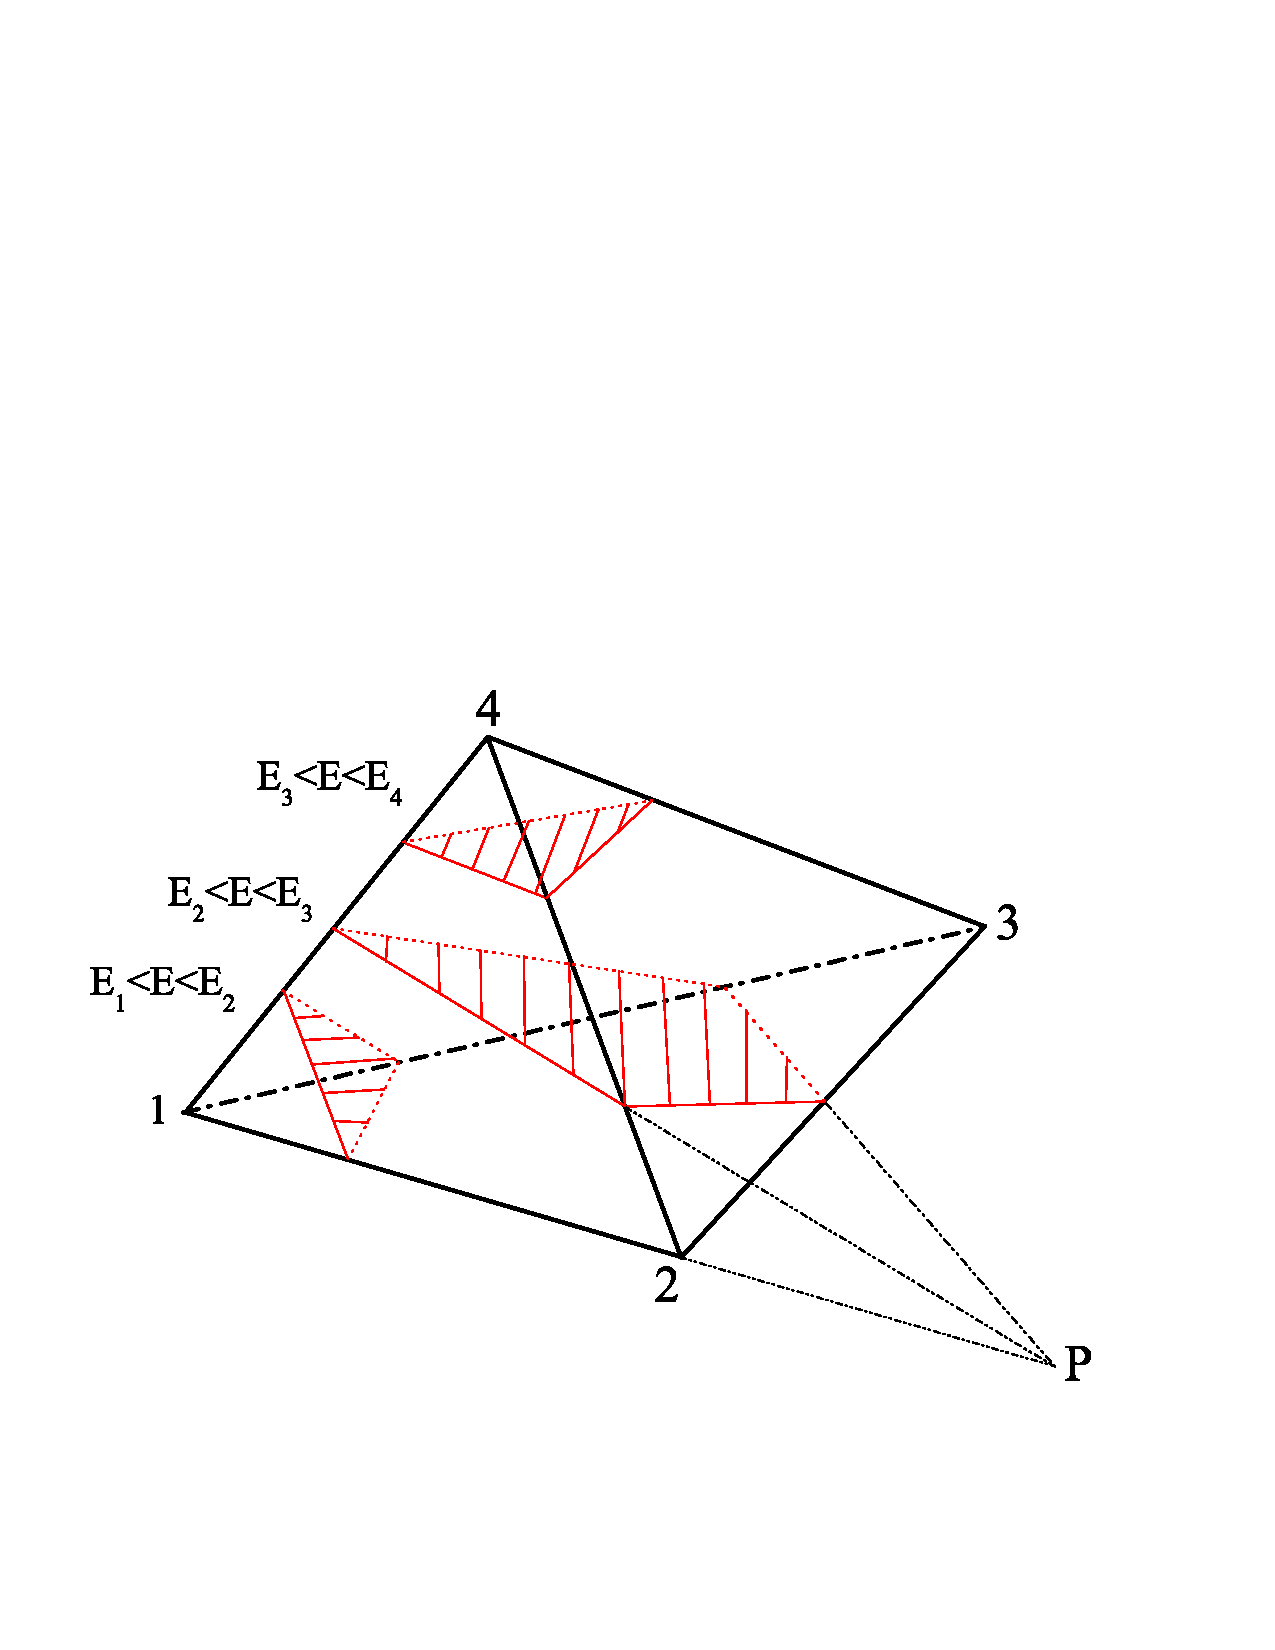
\includegraphics[height=1.28in,width=1.75in,viewport=40 125 525 465,clip]{Figures/Tetra-equal-ene.pdf}}
\label{Specila_Tetrahedron}
\end{figure}
}

\frame
{
\frametitle{四面体布点积分方案}
\begin{itemize}
\setlength{\itemsep}{5pt}
	\item 对\textrm{WS}元胞用$N=(N_1+1)\times(N_2+1)\times(N_3+1)$个网格点(依次编号)分割为$N_1\times N_2\times N_3$个平行六面体
	\item 将每个平行六面体分为4个四面体,记下四面体顶点编号
\end{itemize}
\begin{figure}[h!]
\centering
\hspace*{-10pt}
\vspace*{-10pt}
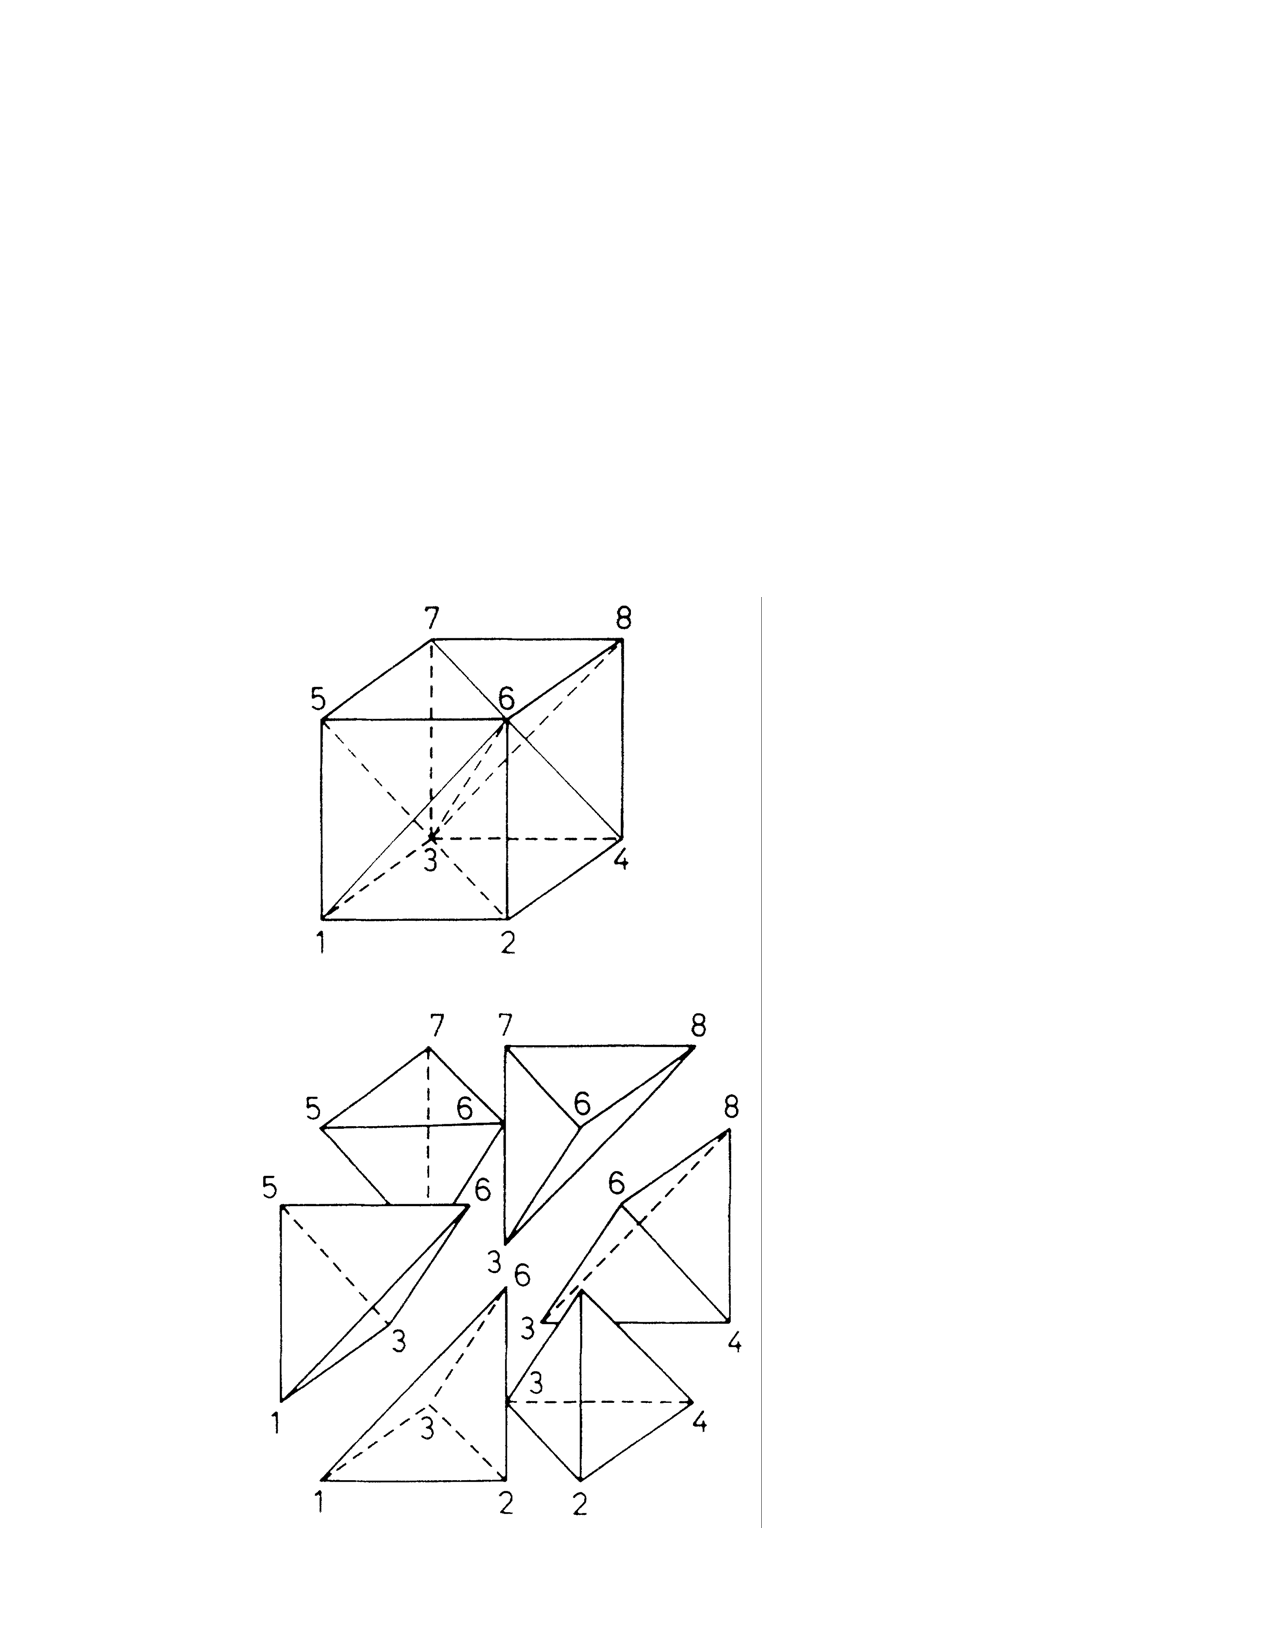
\includegraphics[height=1.8in,width=1.05in,viewport=120 60 360 505,clip]{Figures/submesh_Tetra.pdf}
\caption{\small \textrm{Breakup of a submesh cell into six tetrahedra.}}%(与文献\cite{EPJB33-47_2003}图1对比)
\label{Tetrahedron_split}
\end{figure}

}
\frame
{
\frametitle{四面体布点积分方案}
\begin{itemize}
\setlength{\itemsep}{10pt}
	\item 用点群对称性操作遍历全部网格点,各点对应的不可约第一\textrm{Brillouin}区\textrm{(Irreducible Brillouin zone, IBZ)}等价点标记
	\item 记录不可约\textrm{IBZ}的$\vec k$点及其权重
	\item 四面体中顶点编号全同的归为一类,同时统计各类四面体顶点序号和数目
\end{itemize}
每个四面体对$\vec k$-空间积分的权重表达式可参阅文献\cite{PRB49-16233_1994}
\begin{figure}[h!]
\centering
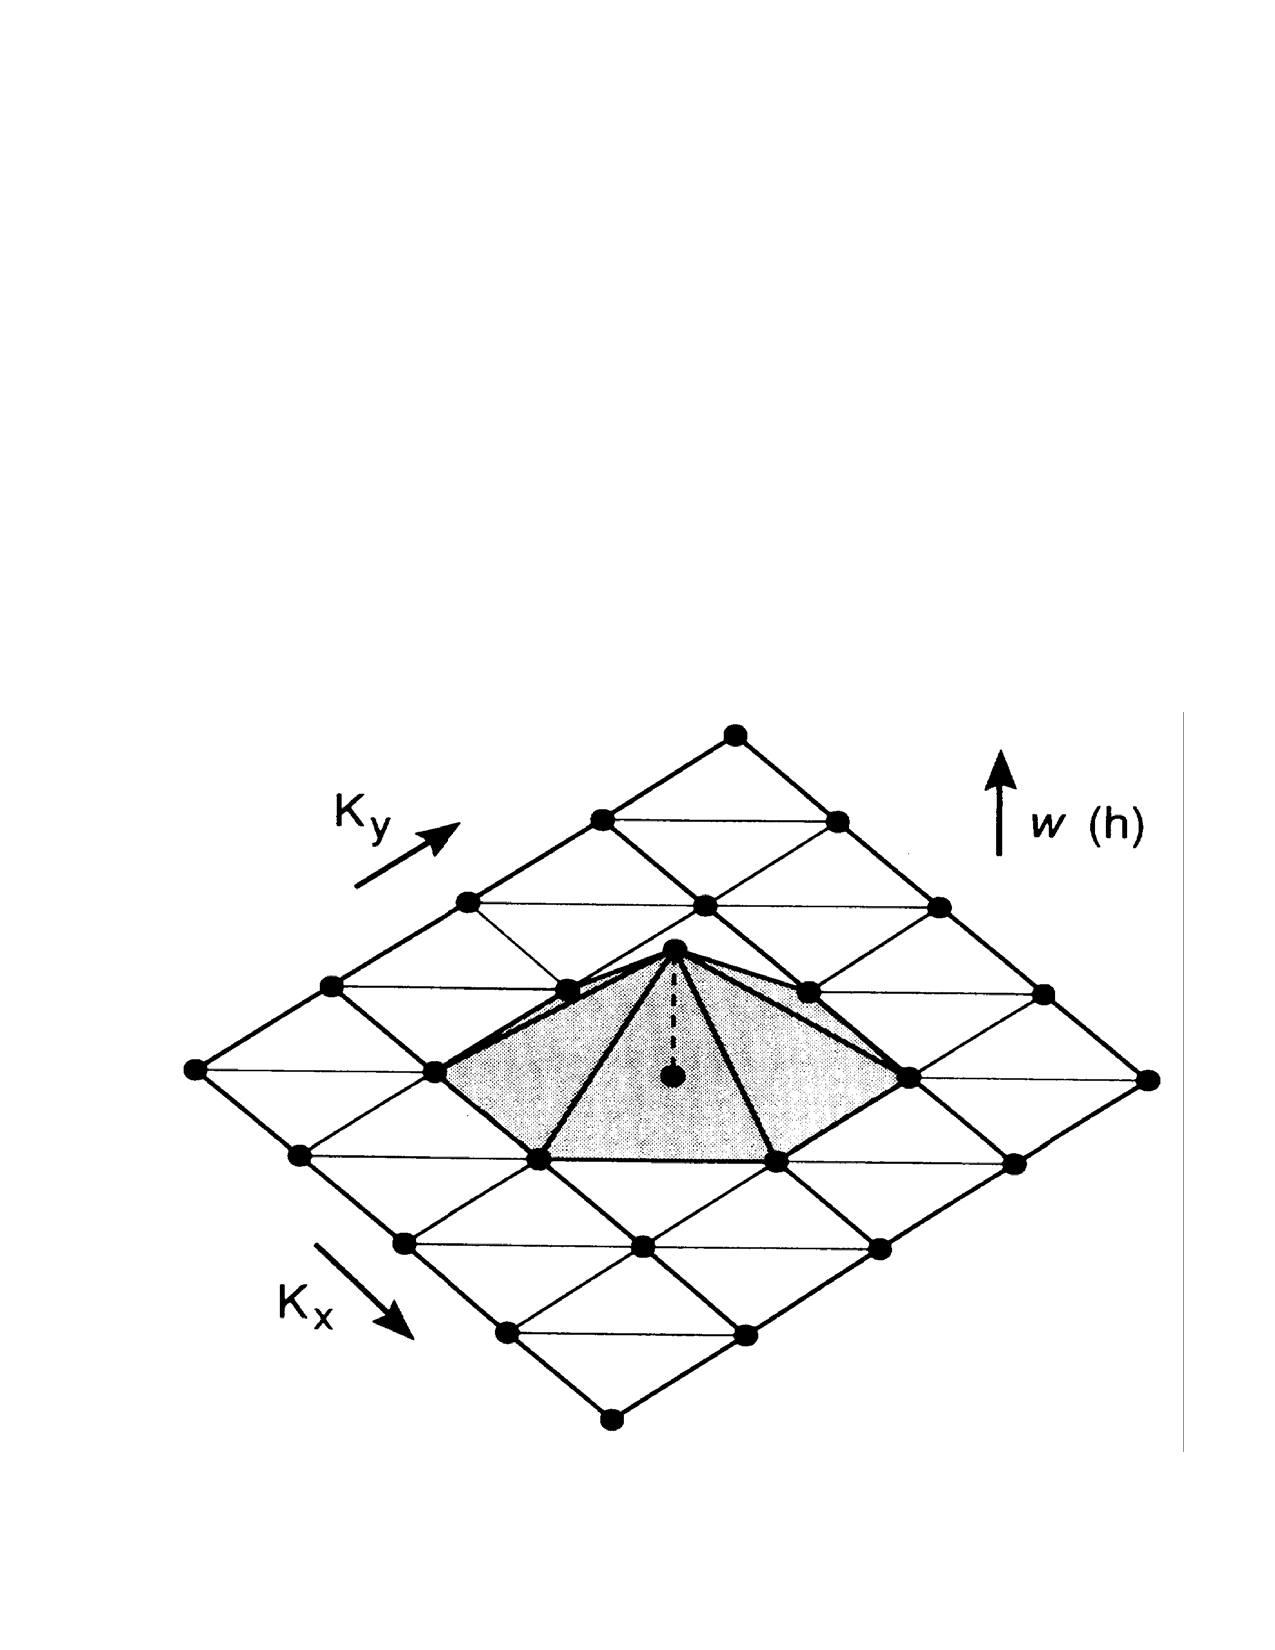
\includegraphics[height=0.95in,width=1.32in,viewport=85 99 560 460,clip]{Figures/dimen_Tetra.pdf}
\caption{\small \textrm{Two-dimensional schematic illustration of the functions $w_j(\vec k)$ that result in the integration weights when integrated.}}%(与文献\cite{EPJB33-47_2003}图1对比)
\label{Tetrahedron_weight}
\end{figure}
}

\section{LDA+$U$与自相互作用的校正}
\frame
{
	\frametitle{\textrm{LDA}+$U$校正的基本思想}
\begin{itemize}
\setlength{\itemsep}{10pt}
	\item 精确密度泛函具有当电子数在整数值前后改变的时候,体系能量的改变是不连续的属性,单电子能量的不连续对能带的带隙有很大贡献
	 \item\textrm{LDA~}近似中体系能量是电子数的连续函数,不具备体系能量随电子数变化不连续的特征。\textrm{LDA/GGA~}方法在描述含有$d$/$f$电子的过渡金属和稀土元素化合物体系时常常失效。
	\item \textrm{LDA}/\textrm{GGA~}得到的体系总能量和实验结果符合较好,但轨道能量(即$\varepsilon_i=\partial E/\partial n_i$),不符合\textrm{Koopmans~}定理,与实验或者严格计算得到的轨道能量差别很大%一个典型的例子就是对H原子的计算结果,LDA计算的轨道能级为$-$0.27\,a.u.(实验结果为$-$0.5\,a.u.),总能量($-$0.488\,a.u.)则非常接近$-$0.5\,a.u.\upcite{PRB37-9919_1988}。
	\item \textrm{Anisimov~}提出通过对\textrm{LDA~}势加入轨道校正克服不足(称为\textrm{LDA+$U$}方法)\upcite{PRB44-943_1991,PRB48-16929_1993}%LDA+U方法与Andersen掺杂模型\upcite{PR124-41_1961}思想类似,
\end{itemize}
}
\frame
{
\frametitle{$U$值的物理含义}
\textrm{$U$}值的物理意义:含有$n$个3$d$\,电子的原子中,\textrm{$U$}值定义为两个原子间转移一个$d$\,电子的能量,即$$2(d^n)\rightarrow d^{n+1}+d^{n-1}$$
\begin{figure}[h!]
\centering
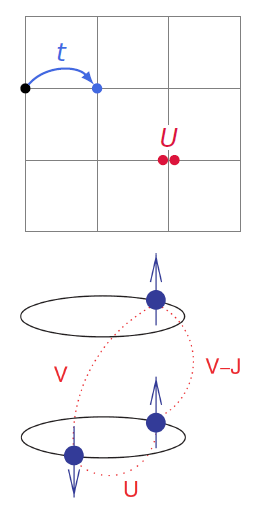
\includegraphics[height=1.35in,width=0.92in,viewport=1 1 240 375,clip]{Figures/LDA_U-1.png}
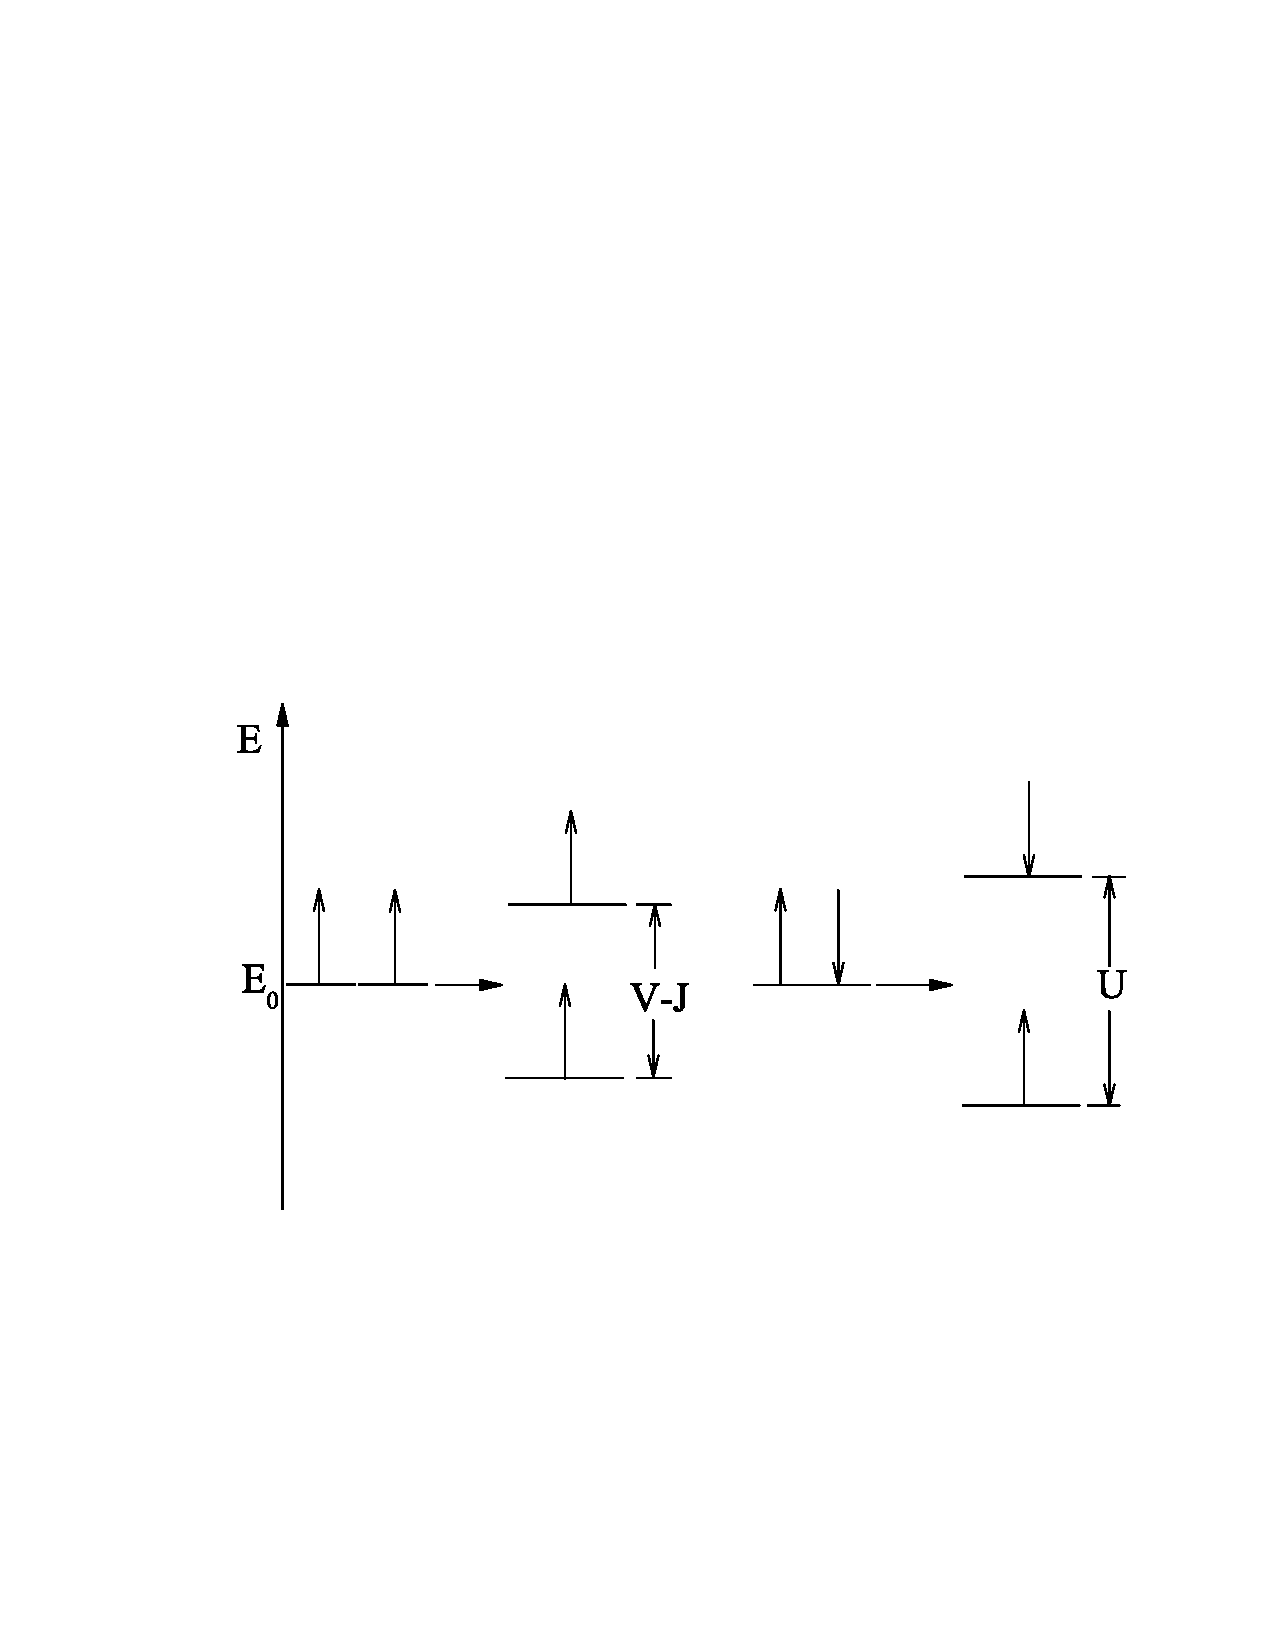
\includegraphics[height=1.35in,width=2.32in,viewport=110 210 545 455,clip]{Figures/LDA_U.pdf}
\caption{\small \textrm{The meaning of $U$, when the Coulomb-interaction of each electron is taken into account.}}%(与文献\cite{EPJB33-47_2003}图1对比)
\label{Tetrahedron_weight}
\end{figure}
}

\section{ABINIT的多体理论}
\frame
{
	\frametitle{\textrm{Green function}与自能}
	\begin{itemize}
		\item 时间序列的\textrm{Green's function}定义为$G(\vec r_1,t_1;\vec r_2,t_2)=-\mathrm{i}\langle\Theta_0^N|\hat{\mathbf{T}}[\hat\psi(\vec r_1,t_1)\hat\psi^{\dag}(\vec r_2,t_2)]|\Theta_0^N\rangle$
		\item \textrm{Green function}的\textrm{Lehmann}表象为$$G(\vec r_1,\vec r_2;\omega)=\sum\limits_i\dfrac{\Psi_i(\vec r_1)\Psi_i^{\dag}(\vec r_2)}{\omega-\varepsilon_i+\mathrm{i}\eta\mathrm{sign}(\varepsilon_i-\mu)}\qquad\eta\rightarrow0^+$$
			由于频率域中时间序列的\textrm{Green's function}包含$(N-1)$个粒子和$(N+1)$个粒子体系的全部激发谱,它们与\textrm{Green's function}在复平面的极值对应
	\end{itemize}
\begin{figure}[h!]
\centering
\vspace{-5pt}
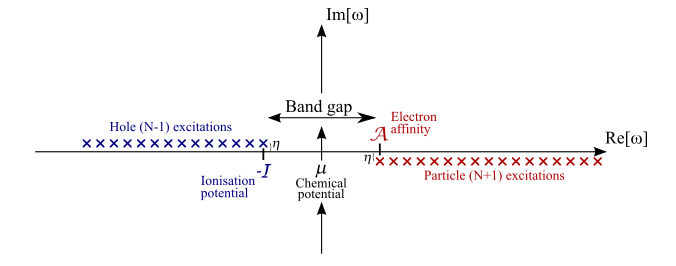
\includegraphics[height=0.80in,width=2.05in,viewport=30 1 660 265,clip]{Figures/GW-0.png}
\caption{\textrm{\small{The poles of the time-ordered Green's function.}}}%(与文献\cite{EPJB33-47_2003}图1对比)
\label{GW-0}
\end{figure}
}

\frame
{
	\frametitle{\textrm{Green function}与自能}
	\textrm{Dyson}方程
	\begin{displaymath}
		\begin{aligned}
	&G(\vec r_1,t_1;\vec r_2,t_2)=G_0(\vec r_1,t_1;\vec r_2,t_2)\\
	&+\int G_0(\vec r_1,t_1;\vec r_3,t_3)\Sigma(\vec r_3,t_3;\vec r_4,t_4)G(\vec r_4,t_4;\vec r_2,t_2)\mathrm{d}t_3\mathrm{d}\vec r_3\mathrm{d}t_4\mathrm{d}\vec r_4
		\end{aligned}
	\end{displaymath}
	\begin{itemize}
		\item \textrm{Dyson}方程描述了相互作用体系$G$通过自能$\Sigma$与近独立体系(传播子)$G_0$关联,自能$\Sigma$是非局域,非\textrm{Hermitian},并与时间相关
		\item 通过求解含有自能$\Sigma$的准粒子方程,可以求解得到多体体系中重整化电子的量子态(\textrm{Hedin}方程)
			$$\bigg[\hat h_0(\vec r_1)+v_H(\vec r_1)\bigg]\Psi(\vec r_1)+\int\Sigma(\vec r_1,\vec r_2;\omega^{\mathrm{QP}})\Psi(\vec r_2)\mathrm{d}\vec r_2=\varepsilon^{\mathrm{QP}}\Psi(\vec r_1)$$
	\end{itemize}
}

\frame
{
	\frametitle{\textrm{Hedin}方程的求解} 
	\textrm{Hedin}方程是积分-微分,可以通过迭代求解
\begin{figure}[h!]
\centering
\vspace{-10pt}
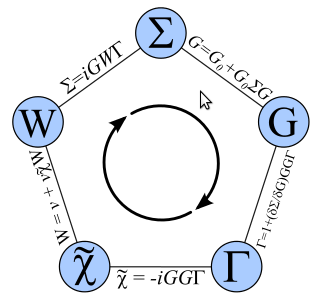
\includegraphics[height=1.0in,width=1.05in,viewport=5 5 330 335,clip]{Figures/GW-1.png}
%\caption{\textrm{\small{The relation of the varibous Green's function.}}}%(与文献\cite{EPJB33-47_2003}图1对比)
\label{GW-1}
\end{figure}
	\begin{itemize}
			\vspace{-15pt}
		\item 定义不可约极化率$\tilde\chi$,$\tilde\chi(\vec r_1,t_1;\vec r_2,t_2)\equiv\dfrac{\delta n(\vec r_1,t_1)}{\delta U_{eff}(\vec r_2,t_2)}=-\mathrm{i}\dfrac{\delta G(\vec r_1,t_1,\vec r_1,t_1+\eta)_{\eta\rightarrow0}}{\delta U_{eff}{\vec r_2,t_2}}$
		\item 定义动态屏蔽相互作用$W(\vec r_1,t_1;\vec r_2,t_2)\equiv\int\epsilon^{-1}(\vec r_1,t_1;\vec r_3,t_3)v(\vec r_3,r_3;\vec r_2,t_2)\mathrm{d}t_3\mathrm{d}\vec r_3$
		\item 介电矩阵与不可约极化率满足关系:
			\begin{displaymath}
				\begin{aligned}
					&\epsilon(\vec r_1,t_1;\vec r_2,t_2)\\
					=&\delta(\vec r_1,t_1;\vec r_2,t_2)-\int v(\vec r_,t_1,\vec r_3,t_3)\tilde\chi(\vec r_3,t_3;\vec r_2,t_2)\mathrm{d}t_3\mathrm{d}\vec r_3
				\end{aligned}
			\end{displaymath}
	\end{itemize}

}

\frame
{
	\frametitle{$GW$近似}
	直接求解\textrm{Hedin}方程是非常复杂的,有必要采取近似(把\textrm{vertex}函数用局域瞬时函数替代),这就是$GW$近似
	$$\Gamma(\vec r_{12},t_{12};\vec r_3t_3)\approx\delta(\vec r_1,t_1;\vec r_2,t_2)\delta(\vec r_1,t_1;\vec r_3,t_3)\equiv\Gamma^{GW}(\vec r_{12},t_{12};\vec r_3,r_3)$$
\begin{figure}[h!]
\centering
\vspace{-15pt}
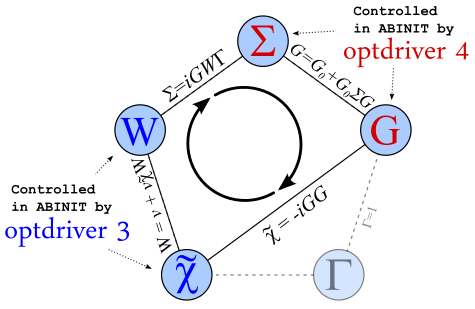
\includegraphics[height=1.0in,width=1.65in,viewport=5 5 530 320,clip]{Figures/GW-3.png}
%\caption{\textrm{\small{The relation of the varibous Green's function.}}}%(与文献\cite{EPJB33-47_2003}图1对比)
\label{GW-2}
\end{figure}
频率空间内,$GW$近似的自能表示为
$$\Sigma(\vec r_1,\vec r_2;\omega)=\dfrac{\mathrm i}{2\pi}\int \mathrm e^{\mathrm i\omega^{\prime}\delta^+}G(\vec r_1,\vec r_2;\omega+\omega^{\prime})W(\vec r_1,\vec r_2;\omega^{\prime})\mathrm{d}\omega^{\prime}$$
}

\frame
{
	\frametitle{由$GW$到$G_0W_0$近似}
	自洽迭代的$GW$方程求解仍然非常复杂,通常选择足够好的近似的$G$和$W$,作单次计算(即$G_0W_0$近似)得到自能
	$$\Sigma(\vec r_1,t_1;\vec r_2,t_2)=\mathrm{i}G_0^{\mathrm{KS}}W_0(\vec r_1,t_1+\eta;\vec r_2,t_2)_{\eta\rightarrow0}$$
	这里$G_0^{\mathrm{KS}}$由独立粒子的\textrm{Kohn-Sham(KS)}Hamiltonian

	屏蔽相互作用由\textrm{KS}本征态能量和波函数的\textrm{RPA}计算的到
	$$\chi^0(\vec r_1,t_1;\vec r_2,t_2)=-\mathrm{i}G_0^{\mathrm{KS}}(\vec r_1,t_1;\vec r_2,t_2)G_0^{\mathrm{KS}}(\vec r_1,t_1;\vec r_2,t_2)$$
	当准粒子波函数用\textrm{KS}轨道近似,本征态$\varepsilon^{\mathrm{KS}}$附近的准粒子能量$\varepsilon^{\mathrm{QP}}$用自能展开
	$$\varepsilon^{\mathrm{QP}}=\varepsilon^{\mathrm{KS}}+Z\langle\Psi^{\mathrm{KS}}|\Sigma(\varepsilon^{\mathrm{KS}}-v_{\mathrm{XC}})|\Psi^{\mathrm{KS}}\rangle$$
	这里重整化因子$Z$定义为$$Z\equiv\bigg[1-\langle\Psi^{\mathrm{KS}}\bigg|\dfrac{\partial\Sigma(\varepsilon)}{\partial\varepsilon^{\mathrm{KS}}}\bigg|\Psi^{\mathrm{KS}}\rangle\bigg]^{-1}$$
}

%\frame
%{
%\frametitle{发展统一理论框架下的材料计算程序}
%\begin{itemize}
%	\item
%\end{itemize}
%}

\appendix
%------------------------------------------------------------------------Reference----------------------------------------------------------------------------------------------
%\begin{thebibliography}{99}
%-----------------------------------------------------------------------------------------------------------------------------------------------------------------------%
%\frame
%{
%\frametitle{主要参考文献}
%{\small
%\bibitem{Singh_Book}\textrm{D. J. Singh. \textit{Plane Wave, PseudoPotential and the LAPW method} (Kluwer Academic, Boston,USA, 1994)}					%
%  \nocite{*}																				%
%}
%}
%\end{thebibliography}
\begin{thebibliography}{99}
\frame
{
\frametitle{主要参考文献}
{\small
\bibitem{PR136-B864_1964}\textrm{P. Hohenberg and W. Kohn \textit{Phys. Rev.} \textbf{136} (1964), B864}
\bibitem{PR140-A1133_1965}\textrm{W. Kohn and L.J. Sham \textit{Phys. Rev.} \textbf{140} (1965), A1133}
\bibitem{Huang_Han}黄昆\:原著、韩汝琦\:改编, {\textit{固体物理学}}\:高等教育出版社, 北京, 1988
\bibitem{Singh_Book}\textrm{D. J. Singh. \textit{Plane Wave, PseudoPotential and the LAPW method} (Kluwer Academic, Boston,USA, 1994)}
\bibitem{PRB41-7892_1990}\textrm{D. Vanderbilt. \textit{Phys. Rev.} B, \textbf{41} (1990), 7892} 
\bibitem{JPCM6-8245_1994}\textrm{G. Kresse and J. Hafner. J. Phys: \textit{Condens. Matter}, \textbf{6} (1994), 8245}
\bibitem{PRB50-17953_1994}\textrm{P. E. Bl\"ochl. \textit{Phys. Rev.} B, \textbf{50} (1994), 17953}
\bibitem{PRB59-1758_1999}\textrm{G. Kresse and D. Joubert \textit{Phys. Rev.} B, \textbf{59} (1999), 1758}
\bibitem{SSC114-15_2000}\textrm{E. Sj\"ostedt, L. Nordstr\"om and D. J. Singh. \textit{Solid State Commun.}, \textbf{114} (2000), 15}
\bibitem{WIEN2k_UG}\textrm{P. Blaha, K. Schwarz, G. Madsen, D. Kvasnicka and J. Luitz. \textit{User's Guide of WIEN2K, An Augmented Plane Wave Plus Local Orbitals Program for Calculating Crystal Properties}. Vienna University of Technology, Inst. of Physical and Theoretical Chemistry, Vienna, Austria (2012)}
\nocite*{}
}
%{\small
%\phantomsection\addcontentsline{toc}{section}{Bibliography}	 %直接调用\addcontentsline命令可能导致超链指向不准确,一般需要在之前调用一次\phantomsection命令加以修正	%
%\bibliography{Myref}																			%
%\bibliographystyle{mybib}																		%
%  \nocite{*}																				%
%}
%-----------------------------------------------------------------------------------------------------------------------------------------------------------------------%
}

\frame
{
\frametitle{主要参考文献}
{\small
%\bibitem{VASP_UG}\textrm{G. Kresse, M. Marsman, and J\"urgen Furthm\"uller. \textit{VASP the GUIDE}. Computational Physics, Faculty of Physics, Universit\"at Wien, Austria (2012) \\url http://cms.mpi.univie.ac.at/VASP/}
\bibitem{Comp_Method}\textrm{V. V. Nemoshkalenko and V. N. Antonov. \textit{Computational Methods in Solid State Physics} (Gordon and Breach Science Publisher, Amsterdam, The Netherlands, 1998)}
\bibitem{JMP22-2433_1981}\textrm{M. Weiner. \textit{J. Math. Phys.}, \textbf{22} (1981), 2433}
\bibitem{PRB26-4571_1982}\textrm{M. Weinert, E. Wimmer and A. J. Freeman. \textit{Phys. Rev.} B, \textbf{26} (1982), 4571}
\bibitem{PRB49-16233_1994}\textrm{P. E. Bl\"ochl, O. Jepsen and O. K. Andersen. \textit{Phys. Rev.} B, \textbf{49} (1994), 16233}
\bibitem{PRB44-943_1991}\textrm{V. I. Anisimov, J. Zaanen and O.K. Andersen. \textit{Phys. Rev.} B, \textbf{44} (1991), 943}
\bibitem{PRB48-16929_1993}\textrm{V.I. Anisimov, I.V. Solovyev, M.A. Korotin, M.T. Czyzyk and G.A. Sawatzky. \textit{Phys. Rev.} B, \textbf{48} (1993), 16929}
\nocite{*}																				%
}
}
\end{thebibliography}
%-----------------------------------------------------------Beamer下不建议使用bib,因为涉及分页--------------------------------------------------------------------------%
%{\small
%\phantomsection\addcontentsline{toc}{section}{Bibliography}	 %直接调用\addcontentsline命令可能导致超链指向不准确,一般需要在之前调用一次\phantomsection命令加以修正	%
%\bibliography{Myref}																			%
%\bibliographystyle{mybib}																		%
%  \nocite{*}																				%
%}

%------------------------------------------------------------------------------------------------------------------------------------------------------------------------------%

\section{$\mathrm{Atompaw}$ 程序包}
\frame
{
	\frametitle{\textrm{Atompaw}程序包简介}
	\textrm{Atompaw}程序包是由\textrm{Holzwarth}、\textrm{Tackett}和\textrm{Matthews}开发的\textrm{PAW}原子数据集生成程序,主要基于基于\textrm{Bl\"ochl}提出的原子数据集生成方案。

	\textrm{Atompaw}程序包产生的原子数据集,主要用于基于\textrm{PAW}方法的材料计算软件\textrm{PWPAW}和\textrm{ABINIT}。

%\centering {\large \textrm{PP-PW}$\Longrightarrow$} \textbf{PP-PAW}$\Longleftrightarrow$\textbf{\textcolor{red}{FP-PAW}}{\large$\Longleftarrow$ \textrm{FP-LAPW}}
%\begin{table}[!H]
%\tabcolsep 5pt 
%%\vspace*{-12pt}
%%\caption{\textrm{The compare of directly diagonalization and $\vec k\cdot\vec p$ perturbation.}}
%\vspace{5pt}
%\label{Table-Compare_CaB6}
%\begin{minipage}{\textwidth}
%%\begin{center}
%\centering
%\def\temptablewidth{1.01\textwidth}
%\rule{\temptablewidth}{1pt}
%\begin{tabular*} {\temptablewidth}{@{\extracolsep{\fill}}cccc}
%	& \textcolor{red}{基函数} & \textcolor{red}{\textrm{Coulomb}势}  &\textcolor{red}{总能量}  \\
%	& \textrm{(PW}与球内分波\textrm{)} & \textrm{(}$\rho_I$与赝电荷$\hat n$\textrm{)}  &奇点排除  \\ \hline
%	\textrm{LAPW}  &\textcolor{blue}{在球面上连续}       &\textcolor{blue}{简单叠加}        & \textcolor{blue}{需要考虑}\\
%	\textrm{PAW}  &\textcolor{blue}{线性变换}:\textcolor{brown}{简单}        &\textcolor{blue}{线性变换}:\textcolor{brown}{复杂}    &\textcolor{blue}{需要考虑}\\
%\end{tabular*}
%\rule{\temptablewidth}{1pt}\\
%%\end{center}
%\end{minipage}
%\end{table}
}

\frame
{
	\frametitle{\textrm{Atompaw}的输入文件}
	\textrm{Atompaw}的输入文件主要包括
	\begin{itemize}
		\item 指定原子名称、核电荷数
		\item 指定交换-相关泛函的形式和径向布点数
		\item 指定原子核外电子的排布(电子组态)
		\item 指定波函数展开所需分波最高角动量和各种半径\\$r_{paw}$、$r_{shape}$、$r_{vloc}$和$r_{core}$
		\item 指定构造外加分波的能量参数$E_l$
		\item 指定\textcolor{blue}{赝波函数、投影子函数(含正交化)和补偿电荷生成方案}
		\item 指定\textcolor{blue}{局域势$v_{loc}(r)$生成方案}
		\item 指定原子数据集输出方式
	\end{itemize}
}

\frame
{
	\frametitle{\textrm{Atompaw}的输出原子数据集文件}
	\textrm{Atompaw}的输出的原子数据集文件主要包括
	\begin{itemize}
		\item 计算中使用的控制参数
		\item 原子价电子波函数$\phi_l(r_i)$
		\item 价电子波函数的赝波函数$\tilde\phi_l(r_i)$
		\item 投影子函数$\tilde p_l(r_i)$
		\item 原子核附近真实价电荷密度$n^1(r_i)$
		\item 赝电荷密度$\tilde n^1(r_i)$
		\item 补充电荷密度$\hat n(r_i)$
		\item 局域势$v_{loc}(r)$
	\end{itemize}
}

\frame
{
	\frametitle{\textrm{Atompaw}程序的计算细节}
	求解原子的价层的全电子分波函数
	$$\hspace*{-62pt}{\footnotesize\bigg(-\dfrac{\hbar^2}{2m}\nabla^2-\dfrac{Ze^2}r+e^2\int\mathrm{d}^3r^{\prime}\dfrac{n_{core}(r^{\prime})+n(r^{\prime})}{|r-r^{\prime}|}+\mu_{XC}[n_{core}(r)+n(r)]\bigg)|\phi_i\rangle=\epsilon_i|\phi_i\rangle}$$
	全电子分波电荷密度
	$$n(r)=\sum_{n,l}c_{n,l}\dfrac{|\phi_{n,l}(r)|^2}{4\pi r^2}$$
}

\frame
{
	\frametitle{\textrm{Atompaw}程序的计算细节}
	有效赝势的构造方案
	\begin{itemize}
		\item \textrm{Troullier-Martin NC} 方案 \\
	首先构造赝波函数满足
	\begin{displaymath}
		\tilde\phi(r)=\left\{
			\begin{aligned}
				&r^{L_v+1}\mathrm{e}^{p(r)}\quad &\mathrm{for}\quad r\leqslant r_c \\
				&\phi(r)\quad &\mathrm{for}\quad r>r_c
			\end{aligned}
			\right.
	\end{displaymath}
	这里$$p(r)=\sum_{m=0}^6C_mr^{2m}$$
	可得赝势 
	$$V_{eff}^{PS}(r)=\epsilon_l+\dfrac{\hbar^2}{2m}\bigg(\dfrac{\mathrm{d}^2p}{\mathrm{d}r^2}+(\dfrac{\mathrm{d}p}{\mathrm{d}r})^2+\dfrac{2(L_v+1)}r\dfrac{\mathrm{d}p}{\mathrm{d}r}\bigg)$$
	于是赝\textrm{Hamiltonian}是$\tilde H(r)=-\dfrac{\hbar^2}{2m}\nabla^2+V_{eff}^{PS}(r)$
	\end{itemize}
}
\frame
{
	\frametitle{\textrm{Atompaw}程序的计算细节}
	有效赝势的构造方案
	\begin{itemize}
		\item \textrm{Ultra-soft} 方案 \\
	构造赝波函数满足
	\begin{displaymath}
		\tilde\phi(r)=\left\{
			\begin{aligned}
				&r^{L_v+1}\sum_{m=0}^3C_mr^{2m}\quad &\mathrm{for}\quad r\leqslant r_c \\
				&\phi(r)\quad &\mathrm{for}\quad r>r_c
			\end{aligned}
			\right.
	\end{displaymath}
	与\textrm{Troullier-Martin NC}方案类似,逆向求解本征方程得到有效赝势
		\item \textrm{Bessel}方案\\
			直接构造有效赝势 $V_{eff}^{PS}(r)=\alpha\cdot\dfrac{\sin(q\cdot r)}r$
	\end{itemize}
}

\frame
{
	\frametitle{\textrm{Atompaw}程序的计算细节}
	赝分波函数与投影子函数构造
	\begin{itemize}
		\item \textrm{Bl\"ochl}方法\\
			构造截断函数$k(r)$
	\begin{displaymath}
		k(r)=\left\{
			\begin{aligned}
				&\bigg[\dfrac{\sin({\pi r/r_c})}{(\pi r/r_c)}\bigg]^2\qquad &\mathrm{for}\quad r<r_c \\
				&0\qquad &\mathrm{for}\quad r\geqslant r_c
			\end{aligned}
			\right.
	\end{displaymath}
	迭代求解方程
	$$(\tilde H(\vec r)-\epsilon_i)|\tilde\phi_i^0(\vec r)\rangle=C_ik(r)|\phi_i^0(\vec r)\rangle$$
	得到初始赝分波$\phi_i^0(\vec r)$\\
	初始投影子函数$|\tilde p_i^0(\vec r)\rangle=\dfrac{k(r)|\tilde\phi_i^0(\vec r)\rangle}{\langle\phi_i^0|k|\phi_i^0\rangle}$
	采用\textrm{Gram-Schmidt}正交化方法正交
	\end{itemize}
}

\frame
{
	\frametitle{\textrm{Atompaw}程序的计算细节}
	赝分波函数与投影子函数构造
	\begin{itemize}
		\item \textrm{Vanderbilt}方法\\
			用多项式构造赝分波函数
	\begin{displaymath}
		\tilde\phi_i(r)=\left\{
			\begin{aligned}
				&r^{l+1}\sum_{m=0}^4C_mr^{2m}\qquad &\mathrm{for}\quad r<r_c \\
				&\phi_l(r)\qquad &\mathrm{for}\quad r\geqslant r_c
			\end{aligned}
			\right.
	\end{displaymath}
	构造辅助函数
	$$\chi_l(r)=\bigg(\epsilon_l+\dfrac{\hbar^2}{2m}(\dfrac{\mathrm{d}^2}{\mathrm{d}r^2}-\dfrac{l(l+1)}{r^2}-V_{eff}^{PS}(r)\bigg)\tilde\phi_l(r)$$
	和变换矩阵\textbf{B},矩阵元$B_{ij}=\int_0^{r_c}\mathrm{d}r\tilde\phi_i(r)\chi_j(r)$
	由此得到投影子函数$\tilde p_i(\vec r)=\sum_{j}\chi_j(r)(\mathbf{B^{-1}})_{ji}$
	\end{itemize}
}


\frame
{
	\frametitle{\textrm{Atompaw}程序的计算细节}
	赝分波函数与投影子函数构造
	\begin{itemize}
		\item \textrm{RRKJ}方法\\
		构造赝分波函数
	\begin{displaymath}
		\tilde\phi_i=\left\{
			\begin{aligned}
				&r\cdot\bigg(\alpha_1^l\cdot j_l(q_1^lr)+\alpha_2^l\cdot j_l(q_2^lr)\bigg) \qquad &\mathrm{for}\quad r<r_c \\
				&\phi_l(r)\qquad &\mathrm{for}\quad r\geqslant r_c
			\end{aligned}
			\right.
	\end{displaymath}
	投影子函数的构造与\textrm{Vanderbilt}方法类似
	\end{itemize}
}


\frame
{
	\frametitle{\textrm{Atompaw}程序的计算细节}
	\begin{itemize}
		\item 赝分波电荷密度的计算
	$$\tilde n(r)=\sum_{n,l}c_{n,l}\dfrac{|\tilde\phi_{n,l}(r)|^2}{4\pi r^2}$$
		\item 赝芯波电荷密度的计算
	\begin{displaymath}
		4\pi r^2\tilde n_{core}(r)=\left\{
			\begin{aligned}
				&r^2(U_0+U_2r^2+U_4r^4)\quad &\mathrm{for}\quad r\leqslant r_c \\
				&4\pi r^2n_{core}(r)\quad &\mathrm{for}\quad r>r_c
			\end{aligned}
			\right.
	\end{displaymath}
	\end{itemize}
}

\frame
{
	\frametitle{\textrm{Atompaw}程序的计算细节}
	\begin{itemize}
		\item 补充电荷的构造
			$$\hat n(r)=\bigg(-Z+\int\mathrm{d}^3r[n_{core}(r)+n(r)-\tilde n_{core}(r)-\tilde n(r)]\bigg)g_{00}(r)$$
			形状函数$g_{LM}$的定义为$$g_{LM}(r)=N_Lr^Lk(r)Y_{LM}(\hat r)$$
			根据$k(r)$的不同可以取\textrm{sinc}、\textrm{Gaussian}或\textrm{Bessel}型等几种
		\item 局域势函数(\textcolor{red}{可移植的“赝势”})
			$$\hspace*{-55pt}\tilde v_{loc}(r)=V_{eff}^{PS}(r)-e^2\int\mathrm{d}^3r^{\prime}\dfrac{\tilde n_{core}(r^{\prime})+\tilde n(r^{\prime})+\hat n(r^{\prime})}{|r-r^{\prime}|}+\mu_{XC}[\tilde n_{core}(r)+\tilde n(r)]$$ 
	\end{itemize}
}

\frame
{
	\frametitle{\textrm{Atompaw}程序的计算细节}
	\begin{itemize}
		\item 相关矩阵元的计算\\
			\textrm{Atompaw}完成了与原子分波、赝分波有关的矩阵元$D_{ij}^{\alpha}$、$O_{ij}^{\alpha}$的\\计算,此外还计算了
			$$W_{ij}^{\alpha}=\sum_{nl}c_{n\vec k}\langle\tilde\Psi_{n\vec k}|\tilde p_i^\alpha\rangle\langle\tilde p_j^{\alpha}|\tilde\Psi_{n\vec k}\rangle$$
			实际计算中,$\tilde\Psi_{n\vec k}$用平面波展开,于是
			$$\hspace*{-20pt}\langle\tilde p_i^{\alpha}|\tilde\Psi_{n\vec k}\rangle=\sqrt{\dfrac1V}\sum_{\vec G}(4\pi \mathrm{i}^l_iY^{\ast}_{l_im_i}(\hat{\vec k+\vec G})\mathrm{e}^{\mathrm{i}(\vec k+\vec G)\cdot\vec R^{\alpha}}\tilde{\tilde p}_{n_il_i}(|\vec k+\vec G|)A_{n\vec k}(\vec G)$$
			这里$$\tilde{\tilde p}_{n_il_i}(\vec q)=\int_0^{r_c^{\alpha}}\mathrm{d}rr\tilde p_{n_il_i}(r)j_{l_i}(\vec q\cdot\vec r)$$
	\end{itemize}
}


\section{适应 $\mathrm{Abinit}$ 的输出}
\frame
{
	\frametitle{\textrm{Atompaw}适应\textrm{Abinit}的输出}
	\begin{itemize}
		\item \textrm{Abinit}程序的\textrm{PAW}计算部分主要基于\textrm{Kresse}和\textrm{Joubert}方案
		\item \textrm{Kresse}方案与\textrm{Bl\"ochl}方案最大的区别在于电荷密度的处理不同
		\item 为了适应\textrm{Abinit}程序包的计算需要,\textrm{Atompaw}提供了专供\\\textrm{Abinit}计算的接口模块\textrm{Abinitinterface},对有关电荷密度与势\\函数作了相应的变换
			$$n_{Z_c}^{\alpha}(|\vec r-\vec R^{\alpha}|)=-Z^{\alpha}\delta(\vec r-\vec R^{\alpha})+n_{core}^{\alpha}(\vec r-\vec R^{\alpha}|)$$
			$$\tilde n_{Z_c}^{\alpha}(|\vec r-\vec R^{\alpha}|)=\tilde n_{core}(|\vec r-\vec R^{\alpha}|)+(-Z^{\alpha}+Q_{core}-\tilde Q_{core})g_{00}(\vec r-\vec R^{\alpha}|)$$
			$${\hat{\hat n}}^{\alpha}(|\vec r-\vec R^{\alpha}|)=\sum_{ij,LM}W_{ij}^{\alpha}G_{l_im_il_jm_j}^{LM}n_{n_il_in_jl_j}^{\alpha L}g_{LM}(\vec r-\vec R^{\alpha})$$
			$$\hspace*{-62pt}\tilde v_{Z_c}^{\alpha}(r)=V_{\alpha}^{PS}(r)-e^2\int\mathrm{d}^3r^{\prime}\dfrac{\tilde n^{\alpha}(r^{\prime})+\hat{\hat{n}}^{\alpha}(r^{\prime})}{|r-r^{\prime}|}+\mu_{XC}[\tilde n_{core}^{\alpha}(r)+\hat{\hat{n}}^{\alpha}(r)+\tilde n^{\alpha}(r)]$$ 
	\end{itemize}
}

%-------------------------------------------------------------------------Thanks------------------------------------------------------------------------------------------------
%\section{致谢}
%\frame
%{
%\frametitle{致$\quad$谢}
%\begin{itemize}
%    \setlength{\itemsep}{20pt}
%  \item 感谢本团队高兴誉、吴泉生、宋红州等各位老师参与的讨论
%  \item 感谢莫所长、宋主任以及软件中心各位老师和同事
%  \item 感谢王崇愚先生的帮助
%\end{itemize}
%}

\logo{}
\frame
{
\vskip 60 pt
%\hskip 10pt \textcolor{blue}{\Huge 感谢答辩委员会各位老师\,\textrm{!}}\\
\vskip 35 pt
\hskip 60pt \textcolor{blue}{\Huge 谢谢大家\:!}
%\vskip 15 pt
%\hskip 40pt \textcolor{blue}{\Huge \textrm{for your attention\:!}}
}

%-------------------------------------------------------------------------------------------------------------------------------------------------------------------------------

\clearpage
%\end{CJK*}
\end{document}
